%%%%%%%%%%%%%%%%%%%%%%%%%%%%%%%%%%%%%%%%%%%%%%%%%%%%%%%%%%%%%%%%%%%%%%%%%%%%%%%
%                       CARREGA DE LA CLASSE DE DOCUMENT                      %
%                                                                             %
% Les opcions admissibles son:                                                %
%      12pt / 11pt            (cos dels tipus de lletra; no feu servir 10pt)  %
%                                                                             %
% catalan/spanish/english     (llengua principal del treball)                 %
%                                                                             % 
% french/italian/german...    (si necessiteu fer servir alguna altra llengua) %
%                                                                             %
% listoffigures               (El document inclou un Index de figures)        %
% listoftables                (El document inclou un Index de taules)         %
% listofquadres               (El document inclou un Index de quadres)        %
% listofalgorithms            (El document inclou un Index d'algorismes)      %
%                                                                             %
%%%%%%%%%%%%%%%%%%%%%%%%%%%%%%%%%%%%%%%%%%%%%%%%%%%%%%%%%%%%%%%%%%%%%%%%%%%%%%%

\documentclass[11pt,spanish,listoffigures,listoftables]{tfgetsinf}

%%%%%%%%%%%%%%%%%%%%%%%%%%%%%%%%%%%%%%%%%%%%%%%%%%%%%%%%%%%%%%%%%%%%%%%%%%%%%%%
%                     CODIFICACIO DEL FITXER FONT                             %
%                                                                             %
%    windows fa servir normalment 'ansinew'                                   %
%    amb linux es possible que siga 'latin1' o 'latin9'                       %
%    Pero el mes recomanable es fer servir utf8 (unicode 8)                   %
%                                          (si el vostre editor ho permet)    % 
%%%%%%%%%%%%%%%%%%%%%%%%%%%%%%%%%%%%%%%%%%%%%%%%%%%%%%%%%%%%%%%%%%%%%%%%%%%%%%%

\usepackage[utf8]{inputenc} 

%%%%%%%%%%%%%%%%%%%%%%%%%%%%%%%%%%%%%%%%%%%%%%%%%%%%%%%%%%%%%%%%%%%%%%%%%%%%%%%
%                        ALTRES PAQUETS I DEFINICIONS                         %
%                                                                             %
% Carregueu aci els paquets que necessiteu i declareu les comandes i entorns  %
%                                          (aquesta seccio pot ser buida)     %
%%%%%%%%%%%%%%%%%%%%%%%%%%%%%%%%%%%%%%%%%%%%%%%%%%%%%%%%%%%%%%%%%%%%%%%%%%%%%%%
\usepackage{amsmath}
\usepackage{tikz}
\usetikzlibrary{positioning}
\usetikzlibrary{babel}
\usepackage{hyperref}
\usepackage{csquotes}
\usepackage{caption}
\usepackage{subcaption}
\newcommand{\mycomment}[1]{}
\usepackage{pdfpages}


%%%%%%%%%%%%%%%%%%%%%%%%%%%%%%%%%%%%%%%%%%%%%%%%%%%%%%%%%%%%%%%%%%%%%%%%%%%%%%%
%                        DADES DEL TREBALL                                    %
%                                                                             %
% titol, alumne, tutor i curs academic                                        %
%%%%%%%%%%%%%%%%%%%%%%%%%%%%%%%%%%%%%%%%%%%%%%%%%%%%%%%%%%%%%%%%%%%%%%%%%%%%%%%

\title{Adaptación de modelos de lenguaje grandes para la generación
de lenguaje natural a partir de palabras clave en sistemas
aumentativos y alternativos de comunicación}
\author{Silvia Alegre Villa}
\tutor{Jorge Civera Saiz}
\curs{2023-2024}

%%%%%%%%%%%%%%%%%%%%%%%%%%%%%%%%%%%%%%%%%%%%%%%%%%%%%%%%%%%%%%%%%%%%%%%%%%%%%%%
%                     PARAULES CLAU/PALABRAS CLAVE/KEY WORDS                  %
%                                                                             %
% Independentment de la llengua del treball, s'hi han d'incloure              %
% les paraules clau i el resum en els tres idiomes                            %
%%%%%%%%%%%%%%%%%%%%%%%%%%%%%%%%%%%%%%%%%%%%%%%%%%%%%%%%%%%%%%%%%%%%%%%%%%%%%%%

\keywords{Aprentatje Automàtic, Transformers, Models de Llenguatge Gran} % Paraules clau 
         {Aprendizaje Automático, Transformers, Modelos de Lenguaje Grandes}              % Palabras clave
         {Machine Learning, Transformers, Large Language Models}        % Key words

%%%%%%%%%%%%%%%%%%%%%%%%%%%%%%%%%%%%%%%%%%%%%%%%%%%%%%%%%%%%%%%%%%%%%%%%%%%%%%%
%                              INICI DEL DOCUMENT                             %
%%%%%%%%%%%%%%%%%%%%%%%%%%%%%%%%%%%%%%%%%%%%%%%%%%%%%%%%%%%%%%%%%%%%%%%%%%%%%%%

\begin{document}

%%%%%%%%%%%%%%%%%%%%%%%%%%%%%%%%%%%%%%%%%%%%%%%%%%%%%%%%%%%%%%%%%%%%%%%%%%%%%%%
%              RESUMS DEL TFG EN VALENCIA, CASTELLA I ANGLES                  %
%%%%%%%%%%%%%%%%%%%%%%%%%%%%%%%%%%%%%%%%%%%%%%%%%%%%%%%%%%%%%%%%%%%%%%%%%%%%%%%

\begin{abstract}
Els Sistemes Augmentatius i Alternatius de Comunicació (SAAC) son eines essencials per a facilitar la comunicació de les persones amb dificultats en la utilització del llenguatge. Aquest sistemes permeten a l'usuari la selecció de pictogrames associats a paraules claus que conformaran l'oració que es desitja comunicar. Posteriorment, aquesta oració pot ser sintetitzada amb veu humana. Els recents avanços en l'àrea del processament del llenguatge natural i, en concret, la proliferació de models de llenguatge grans ofereixen noves perspectives per a millorar els SAAC. En particular, aquest treball explorarà com aquests models de llenguatge poden millorar l'expressivitat de la comunicació dels SAAC quan s'utilitzen per a la generació de llenguatge natural a partir de les paraules clau (pictogrames) seleccionades per l'usuari. D'aquesta manera, aquest treball evaluarà el rendiment d'aquests models quan són adaptats per a la seua integració en els SAAC. Aquesta evaluació es durà a terme utilitzant conjunts de test reals en espanyol i anglés extrets del portal del Centre Aragonés per a la Comunicació Augmentativa i Alternativa.
\end{abstract}
\begin{abstract}[spanish]
 Los Sistemas Aumentativos y Alternativos de Comunicación (SAAC) son herramientas vitales para facilitar la comunicación de las personas con dificultades en la utilización del lenguaje. Estos sistemas permiten al usuario la selección de pictogramas asociados a palabras clave que conformarán la oración que se desea comunicar. Posteriormente, esta oración puede ser sintetizada con voz humana. Los recientes avances en el área del procesamiento de lenguaje natural y, en concreto, la proliferación de modelos de lenguaje grandes ofrece nuevas perspectivas para mejorar los SAAC. En particular, este trabajo explorará cómo estos modelos de lenguaje pueden mejorar la expresividad de la comunicación de los SAAC cuando se utilizan para la generación de lenguaje natural a partir de las palabras clave (pictogramas) seleccionadas por el usuario. De esta forma, este trabajo evaluará el rendimiento de estos modelos cuando son adaptados para su integración en los SAAC. Esta evaluación se llevará a cabo utilizando conjuntos de test reales en español e inglés extraídos del portal del Centro Aragonés para la Comunicación Aumentativa y Alternativa.
\end{abstract}
\begin{abstract}[english]
Augmentative and Alternative Communication (AAC) systems are vital tools for facilitating communication for individuals with difficulties using language. These systems allow users to select pictograms associated with key words that will form the sentence that is wished to communicate. Then, the sentence can be synthesized with a human voice. Recent advances in the field of natural language processing, and specifically the proliferation of large language models, offer new perspectives for improving AAC systems. In particular, this work will explore how these language models can enhance the expressiveness of AAC communication when used to generate natural language from the key words (pictograms) selected by the user. In this way, this work will evaluate the performance of these models when adapted for integration into AAC systems. This evaluation will be carried out using real test sets in spanish and english extracted from the portal of the Aragonese Center for Augmentative and Alternative Communication.
\end{abstract}

%%%%%%%%%%%%%%%%%%%%%%%%%%%%%%%%%%%%%%%%%%%%%%%%%%%%%%%%%%%%%%%%%%%%%%%%%%%%%%%
%                              CONTINGUT DEL TREBALL                          %
%%%%%%%%%%%%%%%%%%%%%%%%%%%%%%%%%%%%%%%%%%%%%%%%%%%%%%%%%%%%%%%%%%%%%%%%%%%%%%%

\mainmatter

%%%%%%%%%%%%%%%%%%%%%%%%%%%%%%%%%%%%%%%%%%%%%%%%%%%%%%%%%%%%%%%%%%%%%%%%%%%%%%%
%                                  INTRODUCCIO                                %
%%%%%%%%%%%%%%%%%%%%%%%%%%%%%%%%%%%%%%%%%%%%%%%%%%%%%%%%%%%%%%%%%%%%%%%%%%%%%%%

\chapter{Introducción} \label{cap1}

En este trabajo se explora cómo los modelos de lenguaje grandes (LLM) pueden ser aplicados en el campo de los Sistemas Aumentativos y Alternativos de Comunicación (SAAC) para la generación de frases de lenguaje natural a partir de palabras clave para su uso en comunicadores electrónicos. Para ello, se entrenarán y evaluarán algunos de los LLM más destacados en la actualidad.

En este primer capítulo se presenta la motivación que impulsa el estudio y los objetivos principales del trabajo, así como una visión general de la estructura que sigue el documento.

\section{Motivación}

La comunicación y el lenguaje son dos pilares fundamentales de la sociedad actual, pues constituyen la base de las relaciones interpersonales, permitiendo el intercambio de ideas e información. Gracias a ello podemos transmitir a los demás nuestros pensamientos, emociones y necesidades, permitiéndonos participar en la vida en sociedad. Sin embargo, para algunas personas el hecho de comunicarse de manera satisfactoria puede suponer un gran desafío. En estos casos, los Sistemas Aumentativos y Alternativos de Comunicación (SAAC) juegan un papel crucial.

Tal y como se explica en el portal del Centro Aragonés para la Comunicación Aumentativa y Alternativa (ARASAAC) \footnote{ARASAAC es un proyecto colaborativo impulsado por el Gobierno de Aragón desde 2007 que ofrece recursos gratuitos y materiales adaptados para mejorar la comunicación y accessibilidad cognitiva de personas que presentan dificultades en estas áreas. Son especialmente conocidos por su banco de pictogramas, ampliamente utilizado en todo el mundo por profesionales, familias y educadores, y ha sido nominado a numerosos premios por su impacto y contribución. Más información en \url{https://arasaac.org}.}, "\textit{los Sistemas Aumentativos y Alternativos de Comunicación (SAAC) son formas de expresión diferentes del lenguaje hablado que tienen como objetivo aumentar el nivel de expresión (aumentativo) y/o compensar (alternativo) las dificultades de comunicación que presentan algunas personas en este área}” \cite{arasaac}.

Existen diversas razones por las cuales una persona podría necesitar utilizar un SAAC. Entre ellas encontramos la parálisis cerebral, la discapacidad intelectual, los trastornos del espectro autista, algunas enfermedades neurológicas, las distrofias musculares o las afasias.

Aunque hay muchos tipos de SAAC, todos se caracterizan por estar basados en sistemas de símbolos, ya sean gráficos (fotografías, dibujos, pictogramas, palabras o letras) o gestuales (mímica o símbolos manuales).

En este trabajo nos centraremos en los comunicadores electrónicos. Los comunicadores electrónicos son herramientas tecnológicas que pueden ser utilizados en cualquier tipo de dispositivo electrónico. Por lo general, consisten en un tablero donde aparecen distintos símbolos gráficos (pictogramas) que representan palabras. Los pictogramas pueden ser organizados y adaptados dependiendo de las necesidades de cada persona, permitiendo que cada usuario añada aquellos que necesite. De esta manera, los usuarios seleccionan secuencias de pictogramas para formar mensajes, que luego son traducidos por el programa en forma de habla digitalizada o texto escrito. Un ejemplo de comunicador electrónico muy utilizado actualmente es el comunicador AsTeRISCS Grid \footnote{El comunicador AsTeRISCS Grid se puede utilizar \textit{online} en \url{grid.asterics.eu}}, desarrollado por ARASAAC, ilustrado en la Figura \ref{fig:comunicador}.

\begin{figure}[h]
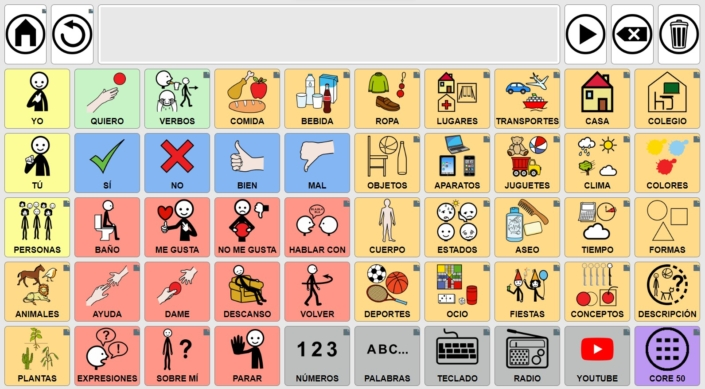
\includegraphics[scale = 0.8]{images/comunicador.jpg}
\centering
\caption{Comunicador AsTeRISCS Grid desarrollado por ARASAAC. Extraído de \cite{asterics_grid_comunicador}}
\label{fig:comunicador}
\end{figure}

Aunque los comunicadores electrónicos son herramientas verdaderamente útiles para mejorar la comunicación de las personas, presentan ciertas limitaciones. Una de las principales es la dificultad para formar frases complejas y gramaticalmente correctas, ya que, para facilitar y simplificar su uso, estos sistemas suelen incluir solamente palabras clave en su forma básica, sin distinguir número, género o tiempo verbal, cosa que restringe en gran medida la fluidez y expresividad de la comunicación.

Algunos de los comunicadores que existen actualmente en el mercado ya emplean diferentes métodos para abordar este problema, pero existe todavía un amplio margen de mejora. Las recientes innovaciones en el campo de la inteligencia artificial y el procesamiento de lenguaje natural ofrecen nuevas oportunidades para superar estas limitaciones. En particular, los modelos de lenguaje grandes tienen un gran potencial para transformar el uso de estos sistemas, pudiendo proporcionar una generación de texto mucho más natural.

\section{Objetivos}

Los objetivos principales de este proyecto son los siguientes:

\begin{enumerate}
	\item Investigar sobre los distintos tipos de Sistemas de Comunicación Aumentativa y Alternativa (SAAC) disponibles, explorando cómo las herramientas de aprendizaje automático e inteligencia artificial podrían optimizar su uso.
	\item Adaptar y evaluar modelos de lenguaje grandes actuales y de acceso público para su implementación  en la generación de frases dentro de herramientas SAAC.
	\item Realizar una comparación de los resultados obtenidos utilizando LLM respecto a otros comunicadores SAAC que permiten la generación de frases y que se encuentran actualmente en el mercado.
\end{enumerate}

\section{Estructura de la memoria}

Este documento está dividido en 6 capítulos. El Capítulo \ref{cap1} proporciona la motivación y los objetivos del trabajo, estableciendo también el contexto de la investigación. El Capítulo \ref{cap2} presenta los conceptos esenciales, comenzando con una visión general del aprendizaje automático y seguido de una explicación detallada de las redes neuronales, tranformers y modelos de lenguaje grandes. En el Capítulo \ref{cap3} se detallan los modelos de lenguaje utilizados, los métodos para su ajuste y adaptación al contexto y las técnicas de evaluación. El Capítulo \ref{cap4} describe los datos utilizados, los experimentos que han sido realizados y los resultados obtenidos. El Capítulo \ref{cap5} ofrece un análisis adicional de los resultados obtenidos con el modelo principal de este proyecto, presentando una comparación de resultados con otros modelos, con resultados de individuos humanos y un análisis de los errores más comunes. Finalmente, el Capítulo \ref{cap6} ofrece un resumen de los resultados, evalúa los objetivos alcanzados y sugiere posibles direcciones para futuras investigaciones.

%\section{Notes bibliografiques} %%%%% Opcional

%????? ????????????? ????????????? ????????????? ????????????? ?????????????

%%%%%%%%%%%%%%%%%%%%%%%%%%%%%%%%%%%%%%%%%%%%%%%%%%%%%%%%%%%%%%%%%%%%%%%%%%%%%%%
%                         CAPITOLS (tants com calga)                          %
%%%%%%%%%%%%%%%%%%%%%%%%%%%%%%%%%%%%%%%%%%%%%%%%%%%%%%%%%%%%%%%%%%%%%%%%%%%%%%%

\chapter{Fundamentos}\label{cap2}

En este capítulo se abordan los conceptos fundamentales necesarios para comprender el funcionamiento de los modelos de lenguaje grandes. En primer lugar, se presenta una visión general del aprendizaje automático, seguido de una explicación detallada sobre las redes neuronales, con un enfoque particular en su aplicación en el procesamiento de texto. A continuación, se explora la arquitectura de los transformers y se presentan los modelos de lenguaje grandes, explicando detalladamente su funcionamiento.

\section{Aprendizaje automático}

El aprendizaje automático (ML, por su nombre en inglés, \textit{machine learning}) es una disciplina dentro de la inteligencia artificial que se centra en el desarrollo y estudio de algoritmos y modelos que permiten que los sistemas puedan realizar tareas específicas sin haber sido explícitamente programados para ello. Este término fue acuñado por Arthur Samuel en el año 1959, quien creo uno de los primeros programas exitosos en esta área, conocido como \textit{the Samuel Ckeckers-playing Program} \cite{samuelCheckers} (el programa de juego de damas de Samuel).

Tom Mitchell \cite{mitchell1997mcgraw} define el proceso de aprendizaje de los programas en el campo del \textit{machine learning} de la siguiente manera:

\begin{displayquote}
\textit{"Se dice que un programa aprende de la experiencia $E$ con respecto a alguna clase de tarea $T$, y medida de rendimiento $P$, si su rendimiento en la tarea $T$, medido por $P$, mejora con la experiencia $E$."}
\end{displayquote}

Aunque la idea principal del aprendizaje automático es esta, encontramos diferentes enfoques dependiendo del tipo de tarea que se quiera llevar a cabo, de la naturaleza de esta, de la medida del rendimiento que se utiliza para evaluar el programa y del tipo de entrenamiento o experiencia que le proporcionamos a este.

Generalmente, los enfoques para el entrenamiento de algoritmos se agrupan en:

\begin{itemize}
	\item \textbf{Aprendizaje supervisado}, cuyo objetivo es, a partir de unos datos de entrenamiento, encontrar la función $f$ que realice el mejor mapeo posible entre un conjunto de entradas $X$ y sus salidas correspondientes $Y$, de manera que $(X, Y) = (X, f(X))$. Para ello, se utilizan datos etiquetados, es decir, datos que incluyen tanto las entradas como las salidas correctas asociadas.
	\item \textbf{Aprendizaje no supervisado}, que trata de modelar la estructura subyacente de un conjunto de datos para identificar relaciones y patrones, permitiendo así un entendimiento más profundo de estos. En este enfoque se utilizan datos no etiquetados.
	\item \textbf{Aprendizaje semisupervisado}, combina elementos del aprendizaje supervisado y el no supervisado, utilizando tanto datos etiquetados como no etiquetados. Este enfoque permite aprovechar la información disponible en grandes volúmenes de datos no etiquetados, utilizando una cantidad menor de datos etiquetados para guiar el proceso de aprendizaje.
	\item \textbf{Aprendizaje por refuerzo}, donde el algoritmo aprende a través de retroalimentaciones que va recibiendo, ajustando sus acciones con el objetivo de maximizar una recompensa acumulada a lo largo del tiempo \cite{mirtaheri2022machine}.

\end{itemize}

La tarea principal de este trabajo se llevará a cabo utilizando técnicas de aprendizaje supervisado.

Otro concepto importante dentro del aprendizaje automático es el aprendizaje profundo (\textit{deep learning}). El aprendizaje profundo es un subconjunto dentro del aprendizaje automático que emplea algoritmos basados en redes neuronales. Dentro de este encontramos métodos como las redes neuronales profundas, las redes neuronales recurrentes, las redes neuronales convolucionales y los transformers, entre otros. Estos métodos tienen aplicaciones significativas en una gran variedad de ámbitos, entre los que se encuentra el procesamiento de lenguaje natural, disciplina en la que se enmarca este trabajo. En las siguientes secciones explicaremos con detalle los conceptos de redes neuronales y transformers.

\section{Redes neuronales} \label{redesNeuronales}

Las redes neuronales son un tipo de modelo que se inspira en la estructura y funcionamiento del cerebro humano para procesar información. El primer modelo de red neuronal artificial fue desarrollado en 1943 por Warren McCulloch y Walter Pitts, y se conoce como \textit{McCulloch-Pitts neuron} \cite{mcculloch1943logical}. Este modelo simplificado imitaba el comportamiento de una neurona natural y marcó el inicio de la investigación en redes neuronales. Aunque las redes neuronales modernas se basan en estas ideas iniciales, han evolucionado significativamente y ya no siguen de manera directa las inspiraciones biológicas originales.

Las redes neuronales modernas están compuestas por pequeñas unidades de cómputo conocidas como neuronas o nodos, conectadas entre sí a través de enlaces para permitir la transmisión de señales entre estas. Los nodos están organizados en capas, de manera que un nodo en una capa está conectado a todos los nodos de la capa siguiente. Existen tres tipos de capa: capa de entrada (\textit{input layer}), capas ocultas (\textit{hidden layers}) y capa de salida (\textit{output layer}). 

La arquitectura más simple de red neuronal es la de perceptrón \cite{RevModPhys.34.123}. Este tipo de modelo surgió como método para la resolución de tareas de clasificación binaria, en las que se debe decidir si una determinada entrada pertenece o no a una clase. Posteriormente, se amplió para abarcar también tareas de clasificación multiclase. Es un tipo de clasificador lineal, por lo que hace sus predicciones basándose en funciones de predicción lineales. Este tipo de arquitectura ha servido como base para arquitecturas de redes neuronales mucho más complejas.

\begin{figure}[h]
	\centering
	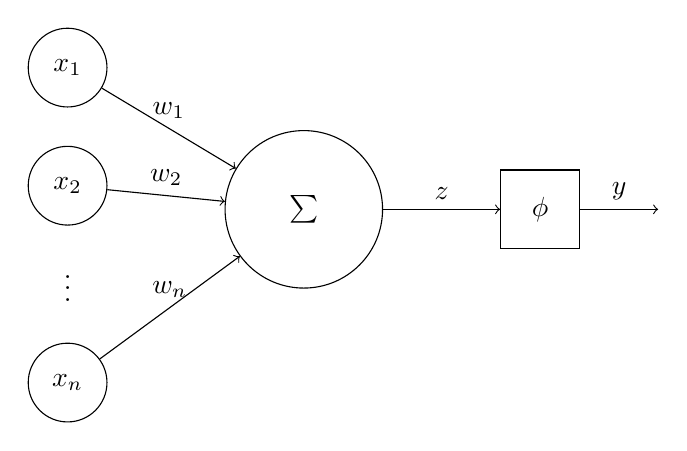
\begin{tikzpicture}
		\tikzstyle{roundnode} = [draw, shape = circle, minimum size = 1cm]
		\tikzstyle{activation} = [draw, shape = rectangle, minimum size = 1cm]
	% Nodos
		\node[roundnode](circle1) at (0, 3.5) {$x_1$};
		\node[roundnode](circle2) at (0, 2) {$x_2$};
		\node (dots) at (0, 0.8) {$\vdots$};
		\node[roundnode](circle3) at (0, -0.5) {$x_n$};

		\node[roundnode, minimum size = 2cm](sum) at (3, 1.7) {$\sum$};
		\node[activation] (act) at (6, 1.7) {$\phi$};

	% Enlaces
		\draw[->]  (circle1) -- (sum) node[midway, above] {$w_1$};
		\draw[->] (circle2) -- (sum) node[midway, above] {$w_2$};
		\draw[->] (circle3) -- (sum) node[midway, above] {$w_n$};
		\draw[->] (sum) -- (act) node[midway, above] {$z$};
		\draw[->] (act) -- (7.5, 1.7) node[midway, above] {$y$};


	\end{tikzpicture}
	\caption{Esquema de perceptrón simple}
	\label{fig:perceptronSimple}	
\end{figure}


Tal y como se observa en la Figura \ref{fig:perceptronSimple}, la arquitectura de perceptrón simple está formada por una única neurona, que toma un vector $x$ como entrada. La neurona calcula la combinación lineal de los elementos del vector $x_1, x_2, ..., x_n$ con los pesos correspondientes $w_1, w_2, ..., w_n$, añadiendo al resultado un valor conocido como umbral o \textit{bias term} $b$. El umbral es una constante que se incorpora para desplazar la función de activación hacia la izquierda o derecha, lo cual puede ser fundamental para el éxito del aprendizaje. Así, la salida producida por la neurona se calcula como:

 \begin{equation}
\label{form:calcularZ}
z = b + \sum_{i = 1}^n w_i x_i
\end{equation}

 A este resultado se le aplica una función $\phi$ conocida como función de activación. Finalmente, se devuelve un solo valor $y$ como salida:

\begin{equation}
y = \phi(z) = 
\begin{cases}
	1 & \text{si } z \ge 0 \\
	0 & \text{si } z < 0
\end{cases}
\end{equation}

El entrenamiento de las redes neuronales consiste en ajustar los vectores de pesos de la red de manera que produzca las salidas más acertadas posibles. En el caso de las redes de perceptrón, al contar con solamente una neurona, este proceso resulta relativamente sencillo. El primer paso es inicializar el vector de pesos con valores aleatorios y calcular la salida de cada vector de entrada del conjunto de entrenamiento. A continuación, se comprueba si la predicción ha sido correcta. Si no lo ha sido, el vector de pesos se modifica utilizando la siguiente fórmula:

\begin{equation}
w = w - \lambda(\hat{y}-y)x
\end{equation}

donde $\lambda$ es el parámetro de tasa de aprendizaje, $\hat{y}$ es el \textit{output} predicho por el modelo y $y$ es la clasificación real. Este proceso se puede realizar muestra a muestra (\textit{online}) o para un subconjunto de muestras de entrenamiento (\textit{batch}).

Así, se repiten estos pasos durante un número determinado de iteraciones o hasta que el modelo converge.

La arquitectura de perceptrón simple tiene una limitación principal, y es que este tipo de modelos solo convergen si las clases en las cuales debe clasificar las muestras son linealmente separables. En caso de que no lo sean, los pesos oscilarán indefinidamente, hasta que el número máximo de iteraciones se alcance. Para solventar esta limitación existen modelos de redes neuronales más complejos, con más neuronas y que utilizan funciones de activación no lineales. El modelo más conocido de este tipo es el de perceptrón multicapa (MLP, por su nombre en inglés \textit{multi-layer perceptron}).

\subsection{Perceptrón multicapa} \label{perceptronmulticapa}

El modelo de perceptrón multicapa es una evolución del modelo de perceptrón simple que tiene como objetivo poder resolver problemas no lineales. La idea principal detrás de este modelo es la combinación de varios perceptrones simples en una única arquitectura más compleja. En esta arquitectura podemos encontrar un número elevado de neuronas, conectadas entre sí y organizadas en capas. Encontramos tres tipos de capas: una capa de entrada (\textit{input layer}), una o más capas ocultas (\textit{hidden layers}) y una capa de salida (\textit{output layer}) (ver Figura \ref{fig:perceptronMulticapa}).

\begin{figure}[h]
    \centering
    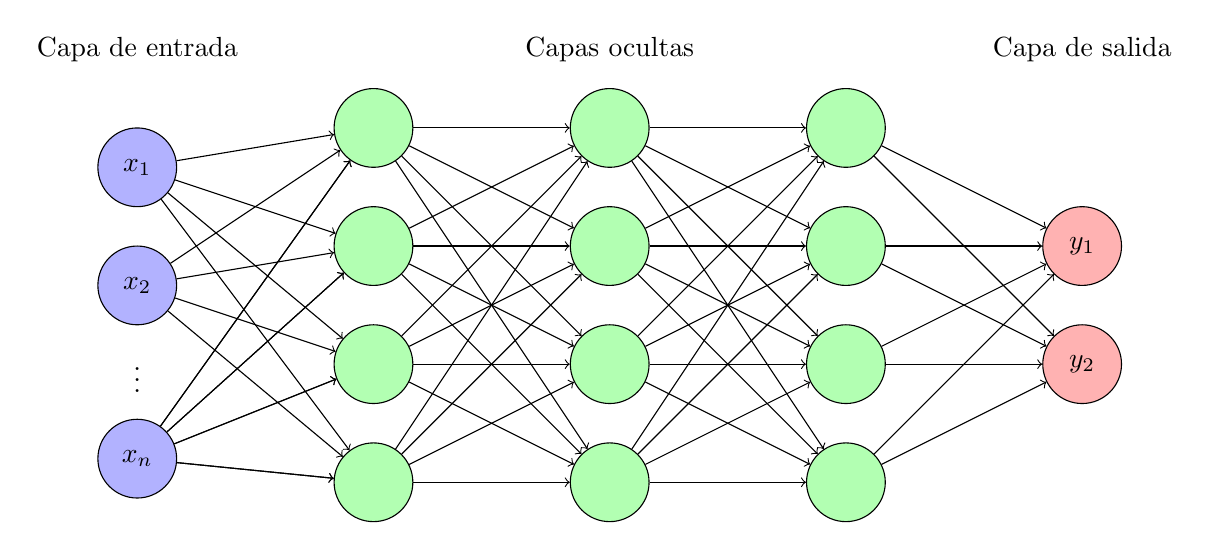
\begin{tikzpicture}
        \tikzstyle{input} = [draw, circle, fill=blue!30, minimum size=1cm]
        \tikzstyle{hidden} = [draw, circle, fill=green!30, minimum size=1cm]
        \tikzstyle{output} = [draw, circle, fill=red!30, minimum size=1cm]
        
        % Nodos de entrada
        \node[input](input1) at (0, 3.5) {$x_1$};
        \node[input](input2) at (0, 2) {$x_2$};
        \node (dots) at (0, 0.9) {$\vdots$};
        \node[input](input3) at (0, -0.2) {$x_n$};

        % Nodos ocultos 1
        \node[hidden](hidden1) at (3, 4) {};
        \node[hidden](hidden2) at (3, 2.5) {};
        \node[hidden](hidden3) at (3, 1) {};
        \node[hidden](hidden4) at (3, -0.5) {};

        % Nodos ocultos 2
        \node[hidden](hidden5) at (6, 4) {};
        \node[hidden](hidden6) at (6, 2.5) {};
        \node[hidden](hidden7) at (6, 1) {};
        \node[hidden](hidden8) at (6, -0.5) {};

        % Nodos ocultos 3
        \node[hidden](hidden9) at (9, 4) {};
        \node[hidden](hidden10) at (9, 2.5) {};
        \node[hidden](hidden11) at (9, 1) {};
        \node[hidden](hidden12) at (9, -0.5) {};

        % Nodos de salida
        \node[output](output1) at (12, 2.5) {$y_1$};
        \node[output](output2) at (12, 1) {$y_2$};

        % Enlaces desde la capa de entrada a la primera capa oculta
        \foreach \i in {1,2,3}
            \foreach \j in {1,2,3,4}
                \draw[->] (input\i) -- (hidden\j);

        \draw[->] (input3) -- (hidden1);
        \draw[->] (input3) -- (hidden2);
        \draw[->] (input3) -- (hidden3);
        \draw[->] (input3) -- (hidden4);
        
        % Enlaces desde la primera capa oculta a la segunda capa oculta
        \foreach \i in {1,2,3,4}
            \foreach \j in {5,6,7,8}
                \draw[->] (hidden\i) -- (hidden\j);

        % Enlaces desde la segunda capa oculta a la tercera capa oculta
        \foreach \i in {5,6,7,8}
            \foreach \j in {9,10,11,12}
                \draw[->] (hidden\i) -- (hidden\j);

        % Enlaces desde la tercera capa oculta a la capa de salida
        \foreach \i in {9,10,11,12}
            \foreach \j in {1,2}
               \draw[->] (hidden\i) -- (output\j);

        % Textos de las capas
        \node at (0, 5) {Capa de entrada};
        \node at (6, 5) {Capas ocultas};
        \node at (12, 5) {Capa de salida};
    \end{tikzpicture}
    \caption{Esquema de perceptrón multicapa}
    \label{fig:perceptronMulticapa}	
\end{figure}

Cada una de las neuronas de una capa está conectada a todas las neuronas de la capa siguiente, y cada uno de los enlaces tiene asociado un peso $w$. De manera similar al modelo de perceptrón simple, los datos se introducen en el modelo en forma de vector a través de la capa de entrada. El ajuste de pesos en el entrenamiento del modelo de perceptrón multicapa se realiza mediante el algoritmo de retropropagación (en inglés, \textit{backpropagation algorithm}) \cite{Rojas1996}. El algoritmo de retropropagación consta de cuatro fases:

\begin{enumerate}
	\item \textbf{Computación hacia adelante (\textit{feed-forward})}: se realiza una pasada hacia adelante a través de la red, desde la capa de entrada hasta la capa de salida. En esta fase, se calculan las salidas de las neuronas utilizando la Ecuación \ref{form:calcularZ} y aplicando sobre este resultado una función de activación no lineal. Algunas de las funciones de activación no lineales más utilizadas son la función sigmoide, la tangente hiperbólica (\textit{tanh}) o la rectificada lineal (\textit{ReLU}). El uso de este tipo de funciones permite que el modelo pueda aplicarse a problemas no lineales. Al llegar a la capa de salida, se calcula la predicción final del modelo.
	\item \textbf{Retropropagación en la capa de salida}: a continuación, se calcula el error en la capa de salida comparando las predicciones del modelo con los valores reales. Posteriormente, se calculan los gradientes del error respecto a los pesos de esta capa.
	\item \textbf{Retropropagación en las capas ocultas}: utilizando los gradientes obtenidos en la capa de salida, el error se propaga hacia atrás a través de las capas ocultas, ajustando los gradientes del error respecto a los pesos en cada una de estas.
	\item \textbf{Actualización de los pesos}: finalmente, se actualizan los pesos de la red utilizando los gradientes calculados en las fases anteriores mediante el método de descenso de gradiente u otro algoritmo de optimización similar.
\end{enumerate}

Este proceso se repite de manera iterativa hasta alcanzar el número máximo de iteraciones o hasta que el modelo converge.

\subsection{Redes neuronales para secuencias de texto}

% Probabilistic neural networks (book1)

El procesamiento de secuencias de texto utilizando redes neuronales es una técnica fundamental en el campo del procesamiento de lenguaje natural. Dado que las redes neuronales operan utilizando vectores numéricos, es necesario transformar las secuencias de texto en vectores de este tipo antes de poder procesarlas. Este proceso se realiza en varias etapas, que se detallan a continuación:

\begin{enumerate}
	\item \textbf{Tokenización y conversión a índices}: el primer paso consiste en descomponer la frase en una secuencia de palabras o tokens. Una vez obtenida la lista de tokens, se asigna a cada uno un número que sirve como índice en un vocabulario.
	\item \textbf{Transformación de palabras en vectores}: los índices numéricos se convierten en vectores utilizando \textit{embeddings}. Los \textit{embeddings} son representaciones vectoriales densas que capturan las características semánticas de las palabras.
	\item \textbf{Creación de la matriz de \textit{embeddings}}: una vez que se han generado los vectores asociados a cada token, se puede construir una matriz de \textit{embeddings} que representa la frase completa. Esta matriz facilita la entrada secuencial de los vectores en la red neuronal.
\end{enumerate}

De esta manera, se consigue una representación en forma de vectores numéricos de las secuencias de texto, de manera que estas puedan ser procesadas por la red neuronal.

En la siguiente sección se presentan las redes neuronales recurrentes (RNN), un tipo de red neuronal que es ampliamente utilizado para el procesamiento de secuencias de texto, y los modelos \textit{encoder-decoder}.

\subsubsection{Redes neuronales recurrentes (RNN)} \label{rnn}
Las redes neuronales recurrentes (RNN, por sus siglas en inglés \textit{recurrent neural networks}) son un tipo de red neuronal diseñadas para procesar secuencias de texto teniendo en cuenta la información aprendida en etapas anteriores. Esto se consigue mediante el mantenimiento de una variable de estado oculto $h_t$, que permite que la predicción $y_t$ depende tanto de la de entrada actual $x_t$ como del estado oculto \cite{murphy2022probabilistic}. El estado oculto $h_t$ es una representación interna de la red en el momento de tiempo $t$, que captura información relevante que ha sido procesada anteriormente y se actualiza a medida que se procesan nuevas entradas.

Las RNN son útiles para tareas como generación de texto, clasificación y traducción de secuencias, ya que pueden capturar dependencias a lo largo del tiempo dentro de los datos secuenciales.

El proceso que siguen este tipo de redes es el siguiente. En primer lugar, se inicializa la red con un estado oculto $h_0$, que puede ser un vector de ceros o una inicialización aprendida. Para cada elemento en la secuencia de entrada, la red actualiza su estado oculto y produce una salida. Así, en el momento de tiempo t, la entrada $x_t$ y el estado oculto previo $h_{t-1}$ se combinan para generar el nuevo estado oculto $h_t$. Este se calcula utilizando la fórmula:

\begin{equation}
h_t = f(W_hh_{t-1} + W_xx_t + b_h)
\end{equation}

donde $W_h$ y $W_x$ son las matrices de pesos asociadas al estado oculto y a las entradas respectivamente, $f$ es una función no lineal y $b_h$ es un vector de sesgos. La salida $y_t$ se obtiene a partir del estado oculto $h_t$:

\begin{equation}
y_t = \phi(W_yh_t + b_y)
\end{equation}

donde $W_y$ es una matriz de pesos, $\phi$ es la función de activación y $b_y$ es un vector de sesgos \cite{sutskever2014sequencesequencelearningneural}.

El proceso se repite para cada elemento de la secuencia de entrada, propagando así la información relevante anterior a través de los estados ocultos.

Uno de los principales problemas de las RNN es la dificultad para recordar información a largo plazo, pues se ha comprobado que, si el modelo es entrenado con secuencias de entrada largas, la importancia de las primeras palabras que son procesadas tiende a ir perdiéndose a medida que se procesa el resto de la secuencia. Esto limita la capacidad de este tipo de redes para capturar dependencias a largo plazo en secuencias largas.

\subsection{Modelos \textit{encoder-decoder}} \label{encdec}

Los modelos \textit{encoder-decoder}, también conocidos como modelos \textit{seq2seq} (\textit{sequence-to-sequence}) son modelos capaces de generar secuencias de salida contextualmente apropiadas a partir de las secuencias de entrada. Estos modelos son capaces de manejar secuencias de longitud variable tanto en la entrada como en la salida. Son modelos ampliamente utilizados en tareas como el resumen de textos, la respuesta a preguntas, la generación de diálogo y la traducción automática \cite{jurafsky2023speech}.

Este tipo de modelos están formados por dos componentes principales: el \textit{encoder} (en español, codificador) y el \textit{decoder} (decodificador). El \textit{encoder} es la primera parte del modelo. Se encarga de transformar las secuencias de entrada a una representación intermedia $h$. Este vector $h$ captura la información relevante de cada elemento de la secuencia de entrada y sus contextos. A continuación, el \textit{decoder} toma el vector de contexto $h$ y, a partir de este, genera la secuencia de salida. Además, el \textit{decoder} puede tener en cuenta también los estados del \textit{encoder} gracias al mecanismo de atención, que se explica en detalle en la Sección \ref{atencion} \cite{sriram2017coldfusiontrainingseq2seq}.

Esta arquitectura se puede implementar utilizando diversos tipos de redes neuronales, incluyendo los transformers, presentados en la Sección \ref{transformers}, o las redes neuronales recurrentes, vistas en el apartado anterior.

\subsection{Atención} \label{atencion}

Tal y como se explicó en la Sección \ref{redesNeuronales}, en las redes neuronales clásicas, el cálculo en cada capa se realiza mediante la combinación lineal de los vectores de entrada y los correspondientes pesos, seguida de la aplicación sobre este resultado de una función de activación. Esta operación se puede representar matemáticamente como $Z = \phi(XW)$, donde $X$ es la matriz formada por los vectores de entrada, $W$ la matriz de pesos, $\phi$ es la función de activación y $Z$ son las salidas de las capas \cite{murphy2022probabilistic}. 

Esta aproximación tiene limitaciones en términos de flexibilidad y capacidad de manejar datos complejos. El mecanismo de atención mejora esto al permitir que los pesos de la red dependan dinámicamente de los datos de entrada. Así, en lugar de utilizar una matriz de pesos fija, el mecanismo de atención ajusta los pesos en función de las características de cada entrada, lo que proporciona una forma más flexible de moldear las relaciones entre la entrada y la salida. Formalmente, esto puede expresarse como $Z = \phi(XW(X))$. Aquí la matriz de pesos ya no es fija, sino que se adapta dinámicamente a la entrada $X$. Esta adaptación permite que el modelo enfoque su atención en diferentes partes de la entrada para cada salida, mejorando su capacidad para capturar información relevante y mejorando su precisión.

De manera más general, el mecanismo de atención puede describirse mediante la fórmula $Z = \phi(VW(Q, K))$. En este contexto:

\begin{itemize}
\item $Q$ (\textit{queries} o consultas) es un conjunto de vectores derivados de $X$ que representan lo que cada palabra "busca" en otras palabras de la secuencia, es decir, con qué otro tipo de palabras puede estar relacionada.
\item $K$ (\textit{keys} o claves) es otro conjunto de vectores también derivado de $X$ que describe las propiedades de cada palabra.
\item $V$ (\textit{values} o valores) es otro conjunto de vectores derivado de $X$ que contiene la información que cada palabra transmite hacia la salida.
\end{itemize}

Estos vectores de \textit{queries}, \textit{keys} y \textit{values} se obtienen procesando las palabras a través de tres redes neuronales independientes.

Cuando se utiliza la atención para calcular una salida $z_i$, se utiliza la \textit{query} $q_i$ correspondiente  y se compara con cada una de las claves $k_j$ de todas las otras palabras de la secuencia, calculando cuál es su nivel de relación con cada una. Esto se realiza mediante el producto escalar entre el vector \textit{query} y los vectores \textit{key} de las otras palabras de la secuencia, de la siguiente manera:

\begin{equation}
\alpha_{ij} = softmax(q_i \cdot k_j)
\end{equation}

Se utiliza la función \textit{softmax} para normalizar los resultados y poder así crear el correspondiente vector. El resultado se representa como $\alpha_{ij}$ y debe cumplir las siguientes condiciones:

\begin{equation}
0 \le \alpha_{ij} \le 1
\end{equation}

\begin{equation}
\sum_j\alpha_{ij} = 1
\end{equation}

El coeficiente $\alpha_{ij}$ determina cuánto peso se debe dar a cada valor $v_j$ en la combinación final, y representa el nivel de importancia que tiene cada palabra de la secuencia sobre la palabra $i$. La salida $z_i$ se calcula entonces como una suma ponderada de los valores $v_j$, donde los pesos son los coeficientes calculados:

\begin{equation}
z_i = \sum_j\alpha_{ij}v_j
\end{equation}

Este enfoque permite que los las salidas del modelo sean una combinación dinámica ponderada de las entradas, lo que hace que este tipo de sistemas sean mucho más efectivos para una amplia gama de tareas, como la traducción automática, el resumen de textos o la generación de texto entre otros \cite{murphy2022probabilistic, jurafsky2023speech}.

\section{Transformers} \label{transformers}

En esta sección se presenta la arquitectura de transformer. Los modelos basados en transformers emplean una arquitectura \textit{encoder-decoder} que utiliza el mecanismo de atención, descrito en la sección anterior. Esta arquitectura fue introducida en el artículo ``\textit{Attention is All You Need}´´ \cite{vaswani2023attentionneed}, publicado en el año 2017, y ha supuesto una gran revolución en diversas áreas del aprendizaje automático por su capacidad para manejar de manera efectiva secuencias largas y complejas \cite{dai2019transformerxlattentivelanguagemodels}. Actualmente, hay una gran cantidad de modelos basados en esta arquitectura que se utilizan en el área del procesamiento de lenguaje natural.

\subsection{Estructura del Transformer}

Tal y como se ha mencionado anteriormente, la arquitectura de transformers utiliza el modelo \textit{encoder-decoder} introducido en la Sección \ref{encdec}. En la estructura del transformer original se utiliza un total de seis bloques de \textit{encoder} y seis de \textit{decoder}, cada uno de los cuales contiene varias capas y mecanismos que facilitan el procesamiento eficiente de las secuencias de datos.

En general, los transformers utilizan tres tipos de capas: capas lineales simples, capas de \textit{multi-head attention} y capas donde encontramos redes neuronales de tipo \textit{feed-forward}. En la Figura \ref{fig:transformers} encontramos el esquema de la estructura de los \textit{encoders} y  \textit{decoders}. Tal y como se puede observar, el \textit{encoder} está formado por una primera capa de \textit{multi-head attention} y, a continuación, una red neuronal de tipo \textit{feed-forward} completamente conectada, además de las capas de normalización que encontramos después de estas. Por lo que respecta al \textit{decoder}, lo conforman dos capas de autoatención y una red neuronal, también con capas de normalización después de estas \cite{jurafsky2023speech, multiheaddotproduct}.

\begin{figure}[h]
    \centering
    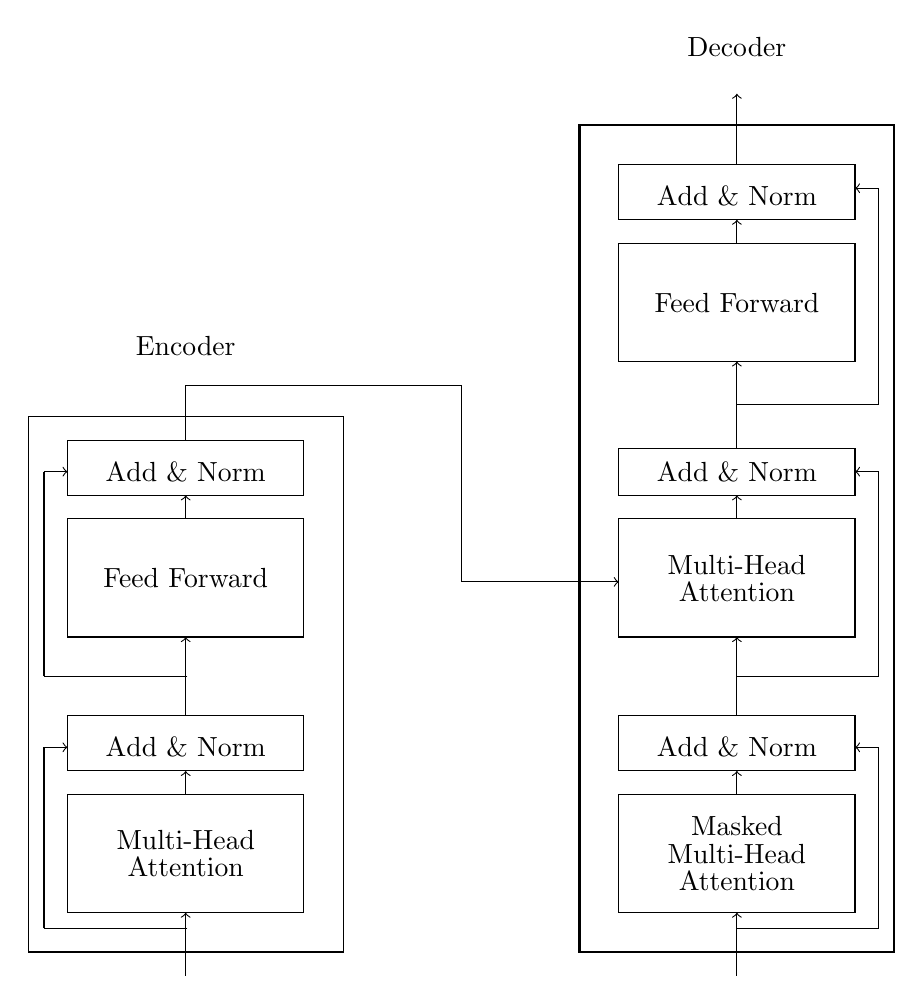
\begin{tikzpicture}[scale=1, transform shape]

        % Encoder
        \draw (0,0) rectangle (4,6.8);
        \node at (2,7.7) {Encoder};
        
        % Encoder components
        \draw (0.5,0.5) rectangle (3.5,2);
        \node at (2,1.25) {\shortstack{Multi-Head\\Attention}};
        
        \draw (0.5,2.3) rectangle (3.5,3);
        \node at (2,2.6) {Add \& Norm};
        
        \draw (0.5,4) rectangle (3.5,5.5);
        \node at (2,4.75) {Feed Forward};
        
        \draw (0.5,5.8) rectangle (3.5,6.5);
        \node at (2,6.1) {Add \& Norm};
        
        % Decoder
        \draw[thick] (7,0) rectangle (11,10.5);
        \node at (9,11.5) {Decoder};
        
        % Decoder components
        \draw (7.5,0.5) rectangle (10.5,2);
        \node at (9,1.25) {\shortstack{Masked\\Multi-Head\\Attention}};
        
        \draw (7.5,2.3) rectangle (10.5,3);
        \node at (9,2.6) {Add \& Norm};
        
        \draw (7.5,4) rectangle (10.5,5.5);
        \node at (9,4.75) {\shortstack{Multi-Head\\Attention}};
        
        \draw (7.5,5.8) rectangle (10.5,6.4);
        \node at (9,6.1) {Add \& Norm};
        
        \draw (7.5,7.5) rectangle (10.5,9);
        \node at (9,8.25) {Feed Forward};
        
        \draw (7.5,9.3) rectangle (10.5,10);
        \node at (9,9.6) {Add \& Norm};
        
        % Encoder lines
	\draw[->] (2, -0.3) -- (2, 0.5);
	\draw[->] (2, 2) -- (2, 2.3);
	\draw[->] (2, 3) -- (2, 4);
	\draw[->] (2, 5.5) -- (2, 5.8);
	\draw (2.02, 0.3) -- (0.2, 0.3);
	\draw (0.2, 0.3) -- (0.2, 2.6);
	\draw[->] (0.2, 2.6) -- (0.5, 2.6);

	\draw (2.02, 3.5) -- (0.2, 3.5);
	\draw (0.2, 3.5) -- (0.2, 6.1);
	\draw[->] (0.2, 6.1) -- (0.5, 6.1);

	% Decoder lines
	\draw[->] (9, -0.3) -- (9, 0.5);
	\draw[->] (9, 2) -- (9, 2.3);
	\draw[->] (9, 3) -- (9, 4);
	\draw[->] (9, 5.5) -- (9, 5.8);
	\draw[->] (9, 6.4) -- (9, 7.5);
	\draw[->] (9, 9) -- (9, 9.3);
	\draw[->] (9, 10) -- (9, 10.9);

	\draw (9, 0.3) -- (10.8, 0.3);
	\draw (10.8, 0.3) -- (10.8, 2.6);
	\draw[->] (10.8, 2.6) -- (10.5, 2.6);

	\draw (9, 3.5) -- (10.8, 3.5);
	\draw (10.8, 3.5) -- (10.8, 6.1);
	\draw[->] (10.8, 6.1) -- (10.5, 6.1); 

	\draw (9, 6.95) -- (10.8, 6.95);
	\draw (10.8, 6.95) -- (10.8, 9.7);
	\draw[->] (10.8, 9.7) -- (10.5, 9.7);


	\draw (2, 6.5) -- (2, 7.2);
	\draw (2, 7.2) -- (5.5, 7.2);
	\draw (5.5, 7.2) -- (5.5, 4.7);
	\draw[->] (5.5, 4.7) -- (7.5, 4.7);

        
    \end{tikzpicture}
    \caption{Esquema de la arquitectura de los transformers}
    \label{fig:transformers}
\end{figure}

La idea principal del transformer es, a lo largo de esta serie de capas, poder construir representaciones contextualizadas cada vez más precisas de los significados de las palabras o tokens de las secuencias de entrada. Así, en las distintas capas del transformer, para obtener la representación de una palabra, se combina la información de la representación obtenida en la capa anterior con la información de las representaciones de las palabras vecinas. El objetivo es producir la versión contextualizada de cada palabra, representando lo que significa esta en el contexto particular en que se encuentra \cite{jurafsky2023speech}.

A continuación se explica con más detalle los procesos que ocurren dentro de cada capa.

\subsection{Capas de \textit{multi-head attention}}
Las capas de \textit{multi-head attention} suponen la verdadera innovación de la arquitectura de transformers \cite{jurafsky2023speech}, pues es en estas donde el modelo aplica el mecanismo de atención.  En este caso, se utiliza una variación del mecanismo de atención explicado en la Sección \ref{atencion}. Esta variación se conoce como \textit{scaled dot-product attention}. Igual que en el mecanismo general de atención, se utilizan tres matrices: la matriz de \textit{queries} $Q$, la de claves $K$ y la de valores $V$. En este caso, el valor de atención se calcula utilizando la siguiente fórmula:

\begin{equation}
A(Q, K, V) = softmax(\frac{QK^t}{\sqrt{d_k}})
\end{equation}

donde $d_k$ es la dimensión del estado oculto de la fuente.

Como vemos, el cambio respecto al cálculo de atención descrito en la Sección \ref{atencion} reside en que en este caso se añade el factor $\frac{1}{\sqrt{d_k}}$, que se utiliza para escalar el resultado obtenido, y conseguir así que las gradientes sean más estables, ya que si la secuencia de entrada fuera muy larga, la función \textit{softmax} puede devolver gradientes extremadamente pequeños, cosa que podría dificultar al modelo realizar un aprendizaje eficiente \cite{multiheaddotproduct}.

De todas maneras, los transformers no se quedan solamente en este concepto, sino que van un paso más allá y utilizan un tipo de atención algo más complejo conocido como \textit{multi-head attention}. Este proceso consiste en calcular distintas atenciones sobre las mismas \textit{queries} y pares clave-valor. Se utiliza este tipo de atención ya que las distintas palabras dentro de la secuencia de texto pueden estar relacionadas entre sí de muchas maneras distintas de manera simultánea. Capturar todas estas relaciones entre palabras es muy complicado si se utiliza un solo valor de atención.

Así, en las capas de \textit{multi-head attention} encontramos distintas capas de atención conocidas como \textit{heads} (cabezas), que calculan valores distintos de atención de manera paralela. Cada una de estas tiene un conjunto distinto de parámetros que se aprende durante el entrenamiento, con los cuales hará el cálculo de atención entre las palabras de entrada. Utilizando parámetros distintos en cada cabeza se consigue que cada una se centre en aspectos distintos de las relaciones entre las palabras. El cálculo de atención para una cabeza $i$ se realiza mediante la siguiente fórmula:

\begin{equation}
H_i = A(QW_i^Q, KW_i^K, VW_i^V)
\end{equation}

donde $W_i^Q$, $W_i^K$ y $W_i^V$ son las matrices de parámetros asociadas a las \textit{queries}, claves y valores, respectivamente, de la cabeza $i$. El valor de \textit{multi-head attention} se obtiene mediante la concatenación de los resultados de las cabezas. Para un total de $h$ cabezas de atención:

\begin{equation}
MultiHead(Q, K, V) = (H_1 \oplus H_2 \oplus ... \oplus H_h)W_O
\end{equation}

La matriz de parámetros $W_O$ proyecta la concatenación de los resultados de las $h$ cabezas de vuelta al subespacio original \cite{cordonnier2021multiheadattentioncollaborateinstead, multiheaddotproduct, jurafsky2023speech}.

\subsection{Capas de redes \textit{feed-forward}}

Las capas \textit{feed-forward} en la arquitectura de transformers están compuestas por redes neuronales independientes de tipo \textit{feed-forward} (en español, redes de propagación hacia adelante). Este tipo de red neuronal es equivalente al modelo de perceptrón multicapa descrito en la Sección  \ref{perceptronmulticapa}.

Así, una red neuronal de tipo \textit{feed forward} es una red multicapa en la que las conexiones entre neuronas no pueden formar ciclos. Esto implica que las señales siempre se propagan en una única dirección: desde la capa de entrada, a través de las capas ocultas, hacia la capa de salida. En la arquitectura de transformers, estas redes están completamente conectadas, lo que significa que las neuronas de una capa reciben las salidas de todas las neuronas de la capa anterior y envían sus salidas a todas las neuronas de la capa siguiente. Además, típicamente contienen solamente una capa oculta.

En los transformers, estas capas complementan las salidas de la capa de atención. Mientras que la capa de atención procesa cada palabra de la secuencia relacionándola con las demás palabras, las capas \textit{feed forward} procesan cada palabra de manera independiente. Este procesamiento independiente es crucial para mejorar la representación de las características extraídas de la capa de atención.

\subsection{Capas de normalización}

Las capas de normalización se encuentran detrás de tanto las capas de atención como las de redes \textit{feed-forward}. En ellas se aplica el proceso de normalización de capas (en inglés, \textit{layer normalization} o \textit{layer norm} \cite{ba2016layernormalization}). Este tipo de normalización se utiliza para mejorar el rendimiento del entrenamiento de redes neuronales profundas, manteniendo los valores de la capa oculta dentro de un rango que facilita el entrenamiento basado en gradientes.

El proceso de normalización de capas toma como entrada un vector para cada palabra de la secuencia, y devuelve este mismo vector normalizado. El primer paso en el proceso es calcular la media $\mu$ y la desviación típica $\sigma$ del vector, de la siguiente manera:

\begin{equation}
\mu^l = \frac{1}{H} \sum_{i = 1}^Hx_i^l
\end{equation}

\begin{equation}
\sigma^l = \sqrt{\frac{1}{H} \sum_{i = 1}^H (x_i^l - \mu^l)^2}
\end{equation}

Donde $H$ es el número de unidades ocultas en la capa. A continuación, los componentes del vector se normalizan restando la media y desviación típica calculadas \cite{jurafsky2023speech}:

\begin{equation}
\hat{x} = \frac{(x - \mu)}{\sigma}
\end{equation}

Finalmente, se introducen parámetros de \textit{bias} $b$ y \textit{gain} $g$:

\begin{equation}
z = g\hat{x} + b
\end{equation}

\section{Modelos de lenguaje grandes} \label{modelosLenguajeGrandes}

Los modelos de lenguaje grandes (LLM por su nombre en inglés, \textit{large language models}) representan una de las innovaciones más significativas en el campo del procesamiento de lenguaje natural. Estos modelos están basados en redes neuronales profundas, y generalmente utilizan la arquitectura de transformers. Estos modelos cuentan con miles de millones de parámetros, y pueden ser entrenados con enormes cantidades de texto, lo que hace que sean capaces de procesar y generar lenguaje humano con una gran fluidez, naturalidad y corrección.

Las tareas sobre las que se aplican son casos de generación condicional, es decir, generación de texto condicionado a un fragmento de entrada, conocido como \textit{prompt}. Así, los LLM son modelos que están diseñados fundamentalmente para predecir la siguiente palabra de una secuencia de palabras \cite{jurafsky2023speech}. Aunque el ámbito de tareas sobre el que se pueden aplicar los LLM pueda parecer reducido, la realidad es que la gran mayoría de tareas en el ámbito de NLP pueden ser enfocadas desde un punto de vista de generación condicional.

En la siguiente sección se explica cómo se deben introducir los datos de entrada al modelo mediante \textit{prompting}.

\subsection{\textit{Prompting}} \label{prompting}

\textit{Prompting} se refiere al proceso mediante el cual se introduce una secuencia de entrada o \textit{query} al modelo, a partir de la cual debe comenzar la tarea de generación de texto. Existen diversas maneras de crear estas \textit{prompts}. Algunas de las técnicas más utilizadas son las siguientes \footnote{Esta  información se ha obtenido de Prompt Engineering Guide \url{www.promptingguide.ai}}:

\begin{itemize}
	\item \textbf{\textit{Zero-shot prompting}}: consiste en presentar al modelo la tarea que se desea realizar sin proporcionar ejemplos previos sobre los que pueda basarse. Los modelos de lenguaje grandes han demostrado funcionar bien con este tipo de \textit{prompting} en tareas simples, aunque pueden tener dificultades en tareas más complejas. En estos casos, puede ser recomendable utilizar \textit{few-shot prompting} en su lugar.
	\item \textbf{\textit{Few-shot prompting}}: en este caso, se proporciona al modelo un número limitado de ejemplos que muestran cómo realizar la tarea. Esta técnica suele ser bastante efectiva,  pero puede fallar en tareas que requieran un razonamiento complejo.
	\item \textbf{\textit{Chain-of-thought} (CoT)} \cite{wei2023chainofthoughtpromptingelicitsreasoning}: esta técnica permite realizar un razonamiento más complejo añadiendo pasos intermedios en la \textit{prompt} que muestren el proceso de pensamiento necesario para resolver el problema. Puede combinarse con \textit{few-shot promting} para tener mejor rendimiento en tareas complejas.
	\item \textbf{\textit{Self-consistency}} \cite{wang2023selfconsistencyimproveschainthought}: consiste en generar diferentes caminos de razonamiento utilizando \textit{few-shot CoT}, y luego seleccionar la respuesta más coherente entre ellos. En esta técnica, el modelo crea varias respuestas posibles y elige la que mejor resuelve el problema.
	\item \textbf{\textit{Tree of thought} (ToT)}:  es una generalización de \textit{CoT prompting} que se basa en la idea de construir un "árbol de pensamientos". Cada pensamiento de este árbol representa un paso intermedio hacia la solución del problema. El modelo evalúa continuamente el progreso a través de estos pasos intermedios y utiliza algoritmos de búsqueda para explorar los diferentes caminos hacia la solución.
\end{itemize}

\subsection{Generación de respuestas}

Una vez introducida la secuencia de entrada en forma de \textit{prompt} al modelo, este debe generar la secuencia de salida. Como se ha mencionado anteriormente, los modelos de lenguaje grandes se utilizan en tareas de generación de texto condicionado a un fragmento de entrada. Es decir, el modelo debe generar un texto de respuesta que esté condicionado a la \textit{prompt} proporcionada.

Para ilustrar este proceso, supongamos que se le introduce al modelo la siguiente \textit{prompt}:

\begin{displayquote}
\centerline{"Pregunta: ¿Cuál es la capital de Francia? Respuesta: "}
\end{displayquote}

A partir de esta, el modelo deberá calcular la probabilidad para cada palabra $w$ dentro de su vocabulario de que esta sea la palabra que continúa la \textit{prompt}:

\begin{displayquote}
\centerline{$P(w|\text{Pregunta: ¿Cuál es la capital de Francia? Respuesta: })$}
\end{displayquote}

Los vocabularios en los LLM se refieren al conjunto de palabras sobre las que trabajan. Así, habiendo calculado las probabilidades para todas las posibles palabras, encontraremos algunas con probabilidades más altas, entre las cuales debería encontrarse la palabra \textit{París}, que es la respuesta a la pregunta. El modelo debería seleccionar esta palabra y, si se quiere generar una respuesta más larga, se calcula la siguiente probabilidad:

\begin{displayquote}
\centerline{$P(w|\text{Pregunta: ¿Cuál es la capital de Francia? Respuesta: París})$}
\end{displayquote}

El proceso puede seguir hasta que lleguemos al número de palabras deseadas.

Inicialmente, este cálculo de probabilidades se realizaba de manera secuencial, basando las predicciones en las distribuciones de probabilidad de las palabras dentro de un texto. Actualmente, se utiliza la arquitectura de transformers, que permite procesar grandes cantidades de texto de manera eficiente y proporciona predicciones mucho más acertadas, pues tiene en cuenta el contexto en el que se encuentran las palabras y las relaciones entre estas \cite{burtsev2023working}.

Existen distintos enfoques para la selección de cuál es la palabra que sigue en la secuencia. Uno de los métodos más simples es utilizar el algoritmo de \textit{greedy decoding} \cite{gu2017trainablegreedydecodingneural}. El algoritmo \textit{greedy decoding} consiste en elegir la palabra $d$ con la probabilidad condicional más alta hasta el momento en cada instante.

\begin{equation}
\hat{d}_i = argmax_{d \in V} P(d | \{d_1, d_2, ..., d_{i-1}\})
\end{equation}

Con el tiempo se ha descubierto que este método llega a resultados subóptimos, pues al elegir siempre la palabra que es más probable que ocurra, tiende a generar textos excesivamente genéricos y repetitivos.

Existe una extensión de este algoritmo conocida como \textit{beam search}, la cual ha demostrado ser más efectiva, sobre todo en tareas de traducción automática. La diferencia entre el algoritmo \textit{greedy decoding} y este, es que el \textit{beam search}, en lugar de quedarse solamente con la palabra con mayor probabilidad y crear una única respuesta, el algoritmo guarda $K > 1$ posibles respuestas (hipótesis) durante la decodificación. Así, en cada iteración, el algoritmo elige las K hipótesis con mayor \textit{score}:

\begin{equation}
p(d_1, d_2, ..., d_N) = \prod_{i = 1}^{N} p(d_i \mid d_1, d_2, ..., d_{i-1})
\end{equation}

Cuando estas se terminan de generar, selecciona la hipótesis con mayor probabilidad.

Aunque el rendimiento de \textit{beam search} es superior al \textit{greedy decoding}, en los LLM se suelen utilizar métodos más complejos, que proporcionan resultados más sofisticados. Estos métodos se conocen como métodos de generación por \textit{sampling}. Se explicarán con detalle en la siguiente sección.

\subsection{Métodos de generación por \textit{sampling}}

En términos generales, el proceso de \textit{sampling} consiste en seleccionar de manera aleatoria una serie de individuos de una muestra, teniendo (o no) en cuenta sus distribuciones de probabilidad. En el contexto de los LLM, esto se traduce en elegir las palabras que se generan en la secuencia de acuerdo con su probabilidad dentro del contexto definido por el modelo. De esta manera, es más probable seleccionar palabras con probabilidades altas y menos probable (aunque no imposible) elegir aquellas con probabilidades bajas.

 El algoritmo de generación por \textit{sampling} más sencillo se conoce como \textit{random sampling}, el cual consiste en seleccionar la siguiente palabra de la secuencia de manera aleatoria según la distribución de probabilidades proporcionada por el transformer. Sin embargo, este enfoque es demasiado simplista para la generación de texto de calidad, ya que al seleccionar las palabras de manera aleatoria, incluso las palabras poco comunes, que tendrán probabilidades bajas, pueden ser elegidas, lo que podría resultar en la generación de frases incorrectas o extrañas \cite{jurafsky2023speech}.

Debido a estas limitaciones, en los LLM se suelen emplear algoritmos más sofisticados, los cuales analizaremos en las siguientes secciones.

\subsubsection{\textit{Top-k sampling}}

El algoritmo de \textit{top-k sampling} es una generalización del \textit{greedy decoding} que consiste en seleccionar las $K$ palabras con mayor probabilidad de la distribución y aplicar \textit{random sampling} únicamente sobre este conjunto. Una vez se seleccionan las $K$ palabras del conjunto, sus probabilidades deben ser normalizadas según el nuevo conjunto. Las probabilidades normalizadas se calculan de la siguiente manera:

\begin{equation}
\hat{p}_i = \frac{p_i * \mathbb{1}\{i \leq K\}}{\sum_{j = 1}^K p_j}
\end{equation}

Donde $\mathbb{1}$ es la función característica, que indica si una palabra está dentro o no del conjunto de las $K$ más probables \cite{nadeem2020systematiccharacterizationsamplingalgorithms}.

\subsubsection{\textit{Nucleus sampling}}

El algoritmo de \textit{nucleus sampling} \cite{holtzman2020curiouscaseneuraltext}, también conocido como \textit{top-p sampling} también sigue la idea de eliminar de la distribución las palabras menos probables. Sin embargo, en lugar de seleccionar un número fijo de palabras, lo que hace es mantener el conjunto de palabras más probables que acumulan una masa de probabilidad $p$. Así, dada una distribución $P(x |x_{1:i-1})$, las \textit{top-p} palabras del vocabulario $V^{(p)} \subset V$ se definen como el conjunto más pequeño que cumpla:

\begin{equation}
\sum_{d \in V^{(p)}} P(d | d_{1:i-1}) \ge p
\end{equation}

Al medir la probabilidad acumulada en lugar de un número fijo de palabras, se espera que esta medida sea más robusta incluso en contextos diversos, que podrían tener resultados muy distintos si se usara un número fijo de palabras. De nuevo, tras seleccionar el subconjunto de palabras del vocabulario se deben normalizar sus probabilidades.

Las probabilidades normalizadas de cada palabra en el vocabulario se pueden calcular como:

\begin{equation}
\hat{p}_i = \frac{p'_i}{\sum_{j:d_j \in V^{(p)}} p'_j}
\end{equation}

Donde $p'_i = p_i * \mathbb{1}\{ d_i \in V^{(p)} \}$ \cite{nadeem2020systematiccharacterizationsamplingalgorithms}.

\subsubsection{\textit{Tempered sampling}}

En el algoritmo de \textit{tempered sampling} \cite{nadeem2020systematiccharacterizationsamplingalgorithms} no crea un subconjunto de palabras del vocabulario, sino que ajusta la distribución de probabilidad de las palabras mediante una transformación. Para ello, se utiliza un parámetro $\tau$, que cumple $0 < \tau < 1$, según la siguiente fórmula:

\begin{equation}
\hat{p}_i = \frac{exp(log(p_i)/\tau)}{\sum_{j = 1}^{|V|}exp(log(p_j)/\tau)}
\end{equation}

Además, existe una variación de este algoritmo que se conoce como \textit{tempered top-k sampling}, el cual combina las transformaciones definidas por el algoritmo \textit{tempered sampling} y el \textit{top-k}. Así, la probabilidad normalizada se calcula:

\begin{equation}
\hat{p}_i = \frac{p'_i}{\sum_{j = 1}^{V^{(k)}}p'_j}
\end{equation}

donde $V^{(k)}$ es el conjunto de las $k$ palabras más probables y $p'_i = exp(log(p_i)/\tau * \mathbb{1}\{i \leq K\}$ .

\subsection{Arquitecturas de los LLM}

Existen cuatro tipos principales de arquitecturas de los LLM:

\begin{itemize}
	\item \textbf{Arquitectura \textit{encoder-decoder}}: esta es la arquitectura explicada en la Sección \ref{encdec}, sobre la cual se basa también la arquitectura de transformers original, presentada en la Sección \ref{transformers}. Tal y como se explicó, consta de un codificador que se encarga de procesar la entrada de texto, transformándola a una representación interna que captura el significado y contexto del texto original. A continuación, el decodificador utiliza esta representación para generar el texto de salida.
	\item \textbf{Arquitectura \textit{encoder-only}}: en esta arquitectura se utiliza únicamente el componente de codificador del modelo \textit{encoder-decoder}. Así, en este enfoque, el codificador crea una representación detallada de la entrada de texto, que puede ser utilizada posteriormente para tareas de comprensión del lenguaje, como la clasificación de texto o la extracción de información.
	\item \textbf{Arquitectura \textit{decoder-only}}: esta arquitectura utiliza únicamente el componente del decodificador. De esta manera, el modelo se entrena para generar texto de manera autorregresiva, es decir, prediciendo cada palabra o token en función de los tokens generados anteriormente. Este enfoque es adecuado para tareas que requieren generación continua de texto, como la completación de frases y la generación de contenido \cite{liu2018generatingwikipediasummarizinglong}.
	\item \textbf{Arquitectura \textit{Mixture of Experts} (MoE)}: introduce un enfoque en el que se utilizan varios expertos especializados para mejorar la eficiencia y el rendimiento del modelo. En lugar de activar todos los parámetros del modelo para cada tarea, solo un subconjunto de expertos se activa en función de la entrada específica. Este enfoque permite una mayor eficiencia en el procesamiento y optimiza el uso de los recursos computacionales.
\end{itemize}

\chapter{Adaptación y evaluación de modelos de lenguaje grandes} \label{cap3}

En este capítulo se presentan los modelos de lenguaje grandes utilizados en este trabajo. Además, se aborda cómo podemos adaptar estos modelos preentrenados para realizar tareas  específicas, explorando las diferentes estrategias y enfoques disponibles. Se hará especial hincapié en el método PEFT  (\textit{parameter-efficient fine-tuning}), centrándonos concretamente en LoRA (\textit{Low-Rank Adaptation}), que es uno de sus tipos de enfoque.

\section{Modelos de lenguaje utilizados} \label{modelosUtilizados}

Para la realización de este trabajo se utilizarán modelos de lenguaje grandes preentrenados. Los modelos de lenguaje grandes preentrenados son modelos que han sido entrenados con grandes cantidades de datos generales, pero que aún no han sido ajustados para realizar tareas específicas. Este tipo de modelos han supuesto una revolución en el campo del procesamiento de lenguaje natural, ya que pueden ser adaptados para realizar una gran variedad de tareas específicas, incluso si estas difieren de los datos originales de entrenamiento. Utilizar LLM preentrenados supone un ahorro de tiempo y recursos significativo, evitando la necesidad de entrenar un modelo desde cero con un gran conjunto de datos.

Algunos de los modelos más utilizados actualmente y que se utilizan en este trabajo son el modelo Gemma, desarrollado por Google, Llama3, desarrollado por Meta, y los modelos GPT, desarrollados por la compañía \textit{OpenAI}. Estos tres modelos se explicarán en detalle en las siguientes secciones.

\subsubsection{Gemma}

Gemma \cite{gemmateam2024gemmaopenmodelsbased} es un modelo de código abierto desarrollado por Google, basado en sus modelos privados Gemini \cite{geminiteam2024geminifamilyhighlycapable}. Existen dos versiones de este modelo: uno con 7 billones de parámetros (modelo 7B), para despliegue en GPU y TPU, y otro con 2 billones (modelo 2B), diseñada para su uso en CPU. El modelo 7B está entrenado con 6T \textit {tokens}, mientras que el 2B, con 3T. En ambos casos, los datos son principalmente en inglés y provienen de documentos web, documentos matemáticos y código. Su entrenamiento se ha realizado mediante \textit{fine-tuning}, utilizando la técnica de  \textit{Reinforcement Learning from Human Feedback} (RLHF) \cite{christiano2023deepreinforcementlearninghuman}.

En cuanto a su arquitectura, esta está basada en el modelo de \textit{transformer decoder only}, pero incorpora varias mejoras significativas:

\begin{itemize}
	\item \textbf{\textit{Multi-Query Attention}} \cite{shazeer2019fasttransformerdecodingwritehead}: es una variación de \textit{multi-head attention} que permite que varias cabezas de las capas de atención compartan las mismas claves y valores, mejorando así la eficiencia computacional.
	\item \textbf{\textit{Rotary Position Embeddings (RoPE)}} \cite{su2023roformerenhancedtransformerrotary}: este tipo de \textit{embeddings} mejora la representación de las posiciones relativas en la secuencia, ya que se basan en la distancia relativa entre los \textit{tokens}.
	\item \textbf{\textit{GeGLU activations}} \cite{shazeer2020gluvariantsimprovetransformer}: en lugar de utilizar la función de activación ReLU, se utiliza la función GeGLU, la cual ha demostrado mejorar el rendimiento del modelo en tareas de generación de texto.
	\item \textbf{Pre-normalización con RMSNorm} \cite{zhang2019rootmeansquarelayer}: se normaliza la entrada a cada una de las capas con RMSNorm para estabilizar el entrenamiento. Este tipo de normalización es más eficiente que la de la arquitectura de transformers original.
\end{itemize}

\subsubsection{LLaMA}

LLaMA \cite{touvron2023llamaopenefficientfoundation} es una familia de modelos de lenguaje \textit{open-source} desarrollados por Meta. Estos modelos van desde los 7B a los 65B de parámetros. Están entrenados utilizando exclusivamente datos disponibles de manera pública, con un conjunto de datos de entrenamiento formado por fuentes diversas, que abarca una gran cantidad de dominios.

En cuanto a su arquitectura, al igual que Gemma, está basada en el modelo de \textit{transformer decoder only}, pero incorpora varias mejoras. Algunas de estas mejoras las encontramos también en los modelos Gemma, como la pre-normalización con RMSNorm o el uso de \textit{rotary position embeddings}. En lugar de la función de activación ReLU, LLaMA utiliza la función SwiGLU \cite{shazeer2020gluvariantsimprovetransformer}, que ha demostrado ser más eficiente en términos de rendimiento del modelo.

LLaMA incorpora también optimizaciones para reducir el tiempo de entrenamiento. Una de estas es la implementación eficiente del \textit{causal multi-head attention}, que consiste en no guardar los valores de los pesos de atención ni calcular los \textit{scores} entre claves y valores que están ocultas en la tarea, reduciendo así el coste computacional. Otra optimización es la reducción de las activaciones recalculadas mediante \textit{checkpointing}, de manera que se guardan las activaciones costosas de calcular implementando manualmente la función hacia atrás para las capas transformadoras.

Concretamente, en este trabajo se utilizará el modelo Llama3.

\subsubsection{Modelos GPT}

Los modelos GPT (\textit{Generative Pre-trained Transformer}) han sido desarrollados por la compañía \textit{OpenAI}, y son una de las familias de modelos de lenguaje de más utilizadas actualmente, especialmente debido a su interfaz de ChatGPT, que ofrece un diseño intuitivo para dar respuesta a preguntas realizadas por los usuarios. En este trabajo se utilizará específicamente el modelo GPT-4.

El modelo GPT-4 \cite{openai2024gpt4technicalreport} es el último de la serie de modelos GPT. La principal innovación de este respecto a sus predecesores es que es un modelo multimodal. Esto significa que, además de aceptar entradas en formato de texto, también es capaz de procesar y analizar imágenes, lo que amplía significativamente su aplicabilidad en una gran variedad de tareas. GPT-4 puede alcanzar resultados a nivel humano en una amplia gama de tareas, tanto en ámbitos profesionales como académicos.

En cuanto a su entrenamiento, este modelo ha sido entrenado con un conjunto de datos mucho más grande que el de sus versiones anteriores. Este conjunto de datos cuenta con más de diez billones de palabras, que es diez veces más que el modelo anterior, GPT-3. Además, los datos utilizados abarcan una amplia variedad de fuentes tanto públicas como proporcionadas por terceros. La técnica utilizada para su entrenamiento fue \textit{fine-tuning} utilizando el método de \textit{Reinforcement Learning from Human Feedback} (RLHF).

Al contrario que los modelos anteriores, este modelo no será reentrenado para su utilización en los experimentos, sino que será utilizado mediante \textit{prompting} desde la interfaz de ChatGPT.

\section{Ajuste de LLM}

Tal y como se ha mencionado en la Sección \ref{modelosUtilizados}, los LLM preentrenados son modelos entrenados con grandes cantidades de datos genéricos que no han sido todavía ajustados para la realización de ninguna tarea específica. Por lo tanto, para aplicarlos a tareas concretas, es necesario ajustar estos modelos para adaptarlos a los requisitos específicos de cada tarea. Generalmente, para adaptar los modelos se utilizan técnicas de \textit{transfer learning}.

\subsection{Aprendizaje por transferencia}

El concepto de aprendizaje por transferencia (en inglés, \textit{transfer learning}) se refiere a la transferencia de conocimiento desde un dominio fuente, donde se dispone de una mayor cantidad de datos, hacia dominios más específicos, que cuentan con menos datos disponibles. Una definición formal dada en \cite{Weiss2016} es la siguiente:

\begin{displayquote}
\textit{"Dado un dominio fuente $D_s$ con una tarea fuente correspondiente $T_s$ y un dominio objetivo $D_t$ con una tarea correspondiente $T_t$, el aprendizaje por transferencia es el proceso de mejora de la función predictiva objetivo $f_t(\cdot)$ mediante el uso de la información relacionada del dominio $D_s$ y la tarea $T_s$, donde $D_s \neq D_t$ o $T_s \neq T_t$"}
\end{displayquote}

Existen cuatro enfoques principales dentro del aprendizaje por transferencia: aprendizaje basado en instancias (\textit{instance-based}), basado en características (\textit{feature-based}), basado en parámetros (\textit{parameter-based}) y basado en relaciones (\textit{relational-based}) \cite{Weiss2016}.

\begin{itemize}
	\item \textbf{Aprendizaje basado en instancias}: la idea principal es utilizar una combinación de modelos preentrenados en el dominio fuente para etiquetar los datos no etiquetados del dominio objetivo. Para ello, se asignan pesos a los modelos del dominio fuente en función de su similitud con el dominio objetivo. Los resultados de los modelos se ponderan según estos pesos para estimar las etiquetas de los datos no etiquetados del dominio objetivo. Finalmente, se construye el modelo del dominio objetivo a partir de los datos etiquetados de este y las etiquetas estimadas.
	\item \textbf{Aprendizaje basado en características}: en este enfoque, se crean nuevos modelos específicos para las tareas, y se incorpora en estos las representaciones obtenidas con el modelo preentrenado, añadiéndolas como características adicionales. De esta manera, el modelo preentrenado sirve como punto de partida para el modelo específico. Utilizando las características extraídas del modelo preentrenado, el modelo específico puede transferir el conocimiento general obtenido por este al contexto del dominio específico de la tarea. Dentro de este enfoque, existen dos variantes: asimétrico y simétrico  \cite{9134370}. En el enfoque asimétrico, se transforma las características extraídas por el modelo preentrenado para que se ajusten a las del dominio objetivo. Por el contrario, en el simétrico lo que se hace es buscar un espacio común de características latentes y transformar tanto las características del dominio fuente como del objetivo en una nueva representación de características.
	\item \textbf{Aprendizaje basado en parámetros}: consiste en modificar y reentrenar el modelo preentrenado para la tarea en particular, ajustando directamente sus parámetros. De esta manera, el modelo conserva el conocimiento general obtenido en el pre entrenamiento y, tras la modificación y reentrenamiento, aprende nuevo conocimiento específico de la tarea.
	\item \textbf{Aprendizaje basado en relaciones}: este enfoque se centra principalmente en los problemas de dominios relacionales, transfiriendo la lógica de relaciones o reglas aprendidas en el dominio fuente al dominio objetivo. Estos métodos buscan preservar y adaptar las relaciones entre entidades para resolver tareas en el nuevo dominio.
\end{itemize}

Para los experimentos de este trabajo, se realizará la adaptación de los modelos de lenguaje preentrenados mediante aprendizaje por transferencia basado en parámetros. Específicamente, se utilizará la técnica de \textit{fine-tuning}.

\section{\textit{Fine-tuning}}

El \textit{fine-tuning} es una técnica dentro del aprendizaje por transferencia basado en parámetros que consiste en ajustar los parámetros del modelo preentrenado utilizando para su entrenamiento un conjunto de datos adaptado a la tarea sobre la que se va a utilizar el modelo.

El principal inconveniente del método de \textit{fine-tuning} es que puede ser un proceso muy lento, ya que es necesario ajustar todos los parámetros del modelo preentrenado, los cuales suelen ser numerosos. Existe un enfoque alternativo en el que se mantiene el modelo preentrenado intacto, y se añaden unos pocos parámetros adicionales que modifican su comportamiento interno para adaptarlo a la tarea específica. Durante el entrenamiento, solamente es necesario ajustar estos nuevos parámetros. Esta idea se conoce como adaptadores.

\subsection{Adaptadores}

El método de ajuste basado en adaptadores funciona añadiendo módulos específicos a un modelo preentrenado, de manera que durante el entrenamiento de este para alguna tarea específica se actualizan únicamente los parámetros de estos módulos, y no los del modelo completo. De esta manera, se incorporan solo unos pocos parámetros entrenables para cada nueva tarea, lo que permite un alto grado de compartición de parámetros \cite{he2021effectivenessadapterbasedtuningpretrained}. Este enfoque puede ser utilizado como alternativa al \textit{fine-tuning} completo del modelo, ya que, se ha demostrado que ambos métodos ofrecen un rendimiento comparable, siendo el ajuste con adaptadores mucho más eficientes en términos del número parámetros \cite{houlsby2019parameterefficienttransferlearningnlp, stickland2019bertpalsprojectedattention}.

Los módulos de los adaptadores deben cumplir con dos propiedades esenciales: contener un número reducido de parámetros y tener una inicialización cercana a la identidad. Los adaptadores deben ser pequeños en comparación con las capas del modelo original para asegurar que el modelo crezca de manera controlada al añadir nuevas tareas. La inicialización cercana a la unidad es necesaria para mantener la estabilidad del entrenamiento. De esta manera, el modelo original no se verá afectado al inicio del entrenamiento. Durante este, los adaptadores pueden activarse para cambiar la distribución de las activaciones en la red. Además, los módulos pueden ignorarse si no son necesarios. Si la inicialización se desviara demasiado de la identidad, el modelo podría fallar durante el entrenamiento \cite{houlsby2019parameterefficienttransferlearningnlp}.

En el ámbito del procesamiento de lenguaje natural, los adaptadores generalmente se insertan como módulos entre las capas del modelo. En el caso de la arquitectura de transformers, la idea es insertar dos redes neuronales MLP poco profundas como cuello de botella dentro de cada uno de los bloques del transformer: una después de la capa de \textit{multi-head attention} y otra, después de la capa de red \textit{feed forward}. Estas redes MLP deben tener lo que se conoce como \textit{skip connections}, es decir, conexiones que permiten saltarse capas intermedias, para permitir la inicialización de las redes como identidad \cite{murphy2022probabilistic}.

\section{\textit{Parameter-efficient fine-tuning} (PEFT)}

El \textit{Parameter- Efficient Fine-Tuning} (PEFT) es uno de los métodos de ajuste basados en adaptadores que pueden aplicarse a modelos de lenguaje grandes. Este método incluye cuatro enfoques: basado en \textit{promtps}, basado en reparametrización, adaptadores en serie y adaptadores en paralelo.

En este trabajo, se empleará el enfoque basado en reparametrización. Este se centra en la transformación de los pesos de la red mediante técnicas de bajo rango, de manera que se consigue reducir de manera eficaz el número de parámetros que necesitan ser entrenados, mientras se conserva la capacidad de manejar matrices de alta dimensión \cite{hu2023llmadaptersadapterfamilyparameterefficient}. Dentro de este marco, existen varios métodos, entre los cuales se destaca LoRA (\textit{Low-Rank Adaptation}), que es el enfoque que se utilizará en este proyecto.

\subsection{\textit{Low-Rank Adaptation} (LoRA)} \label{lora}

El método de \textit{Low-Rank Adaptation} (LoRA) fue presentado en el artículo \textit{LoRA: Low-Rank adaptation of Large Language models} \cite{hu2021loralowrankadaptationlarge}, desarrollado por un equipo de Microsoft. Como se mencionó en la sección anterior, este forma parte del enfoque PEFT basado en reparametrización de los modelos. LoRA se basa en congelar los pesos del modelo preentrenado durante el entrenamiento para luego ajustarlos mediante una matriz de parámetros adicionales que representan el cambio necesario en los pesos originales del modelo. La matriz de cambios es la que se ajusta en el entrenamiento. Generalmente, la matriz de pesos originales se denota como $W$ y la matriz de cambios, $\bigtriangleup W$.

\begin{figure}[!h]
\centering
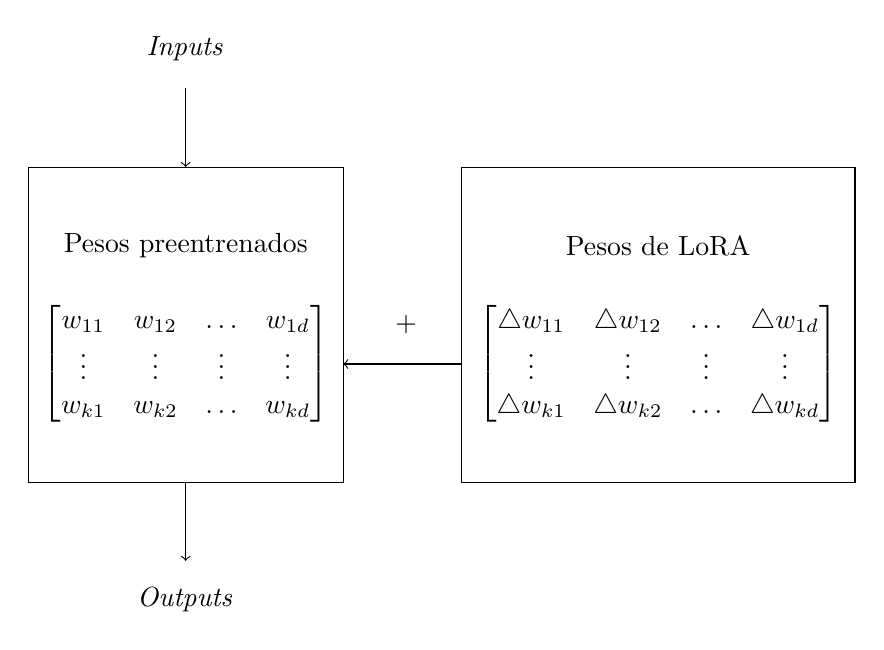
\begin{tikzpicture}

% Modelo preentrenado
\draw (0,0) rectangle (4,4);
\node at (2,3) {Pesos preentrenados};
\node at (2, 1.5) {
\(\begin{bmatrix}
w_{11} & w_{12} & \dots & w_{1d} \\
\vdots & \vdots & \vdots & \vdots \\
w_{k1} & w_{k2} & \dots & w_{kd}
\end{bmatrix}\)
};

% LoRA
\draw (5.5,0) rectangle (10.5,4);
\node at (8,3) {Pesos de LoRA};
\node at (8, 1.5) {
\(\begin{bmatrix}
\bigtriangleup  w_{11} & \bigtriangleup  w_{12} & \dots & \bigtriangleup w_{1d} \\
\vdots & \vdots & \vdots & \vdots \\
\bigtriangleup w_{k1} & \bigtriangleup w_{k2} & \dots & \bigtriangleup w_{kd}
\end{bmatrix}\)
};

% Flechas
\node at (2, 5.5) {\textit{Inputs}};
\draw[->] (2,5) -- (2,4);

\node at (2, -1.5) {\textit{Outputs}};
\draw[->] (2, 0) -- (2, -1);

\draw[->] (5.5, 1.5) -- (4, 1.5);
\node at (4.8, 2) {+};
\end{tikzpicture}
\caption{Esquema de las matrices de parámetros de LoRA}
\label{fig:matricesLoRA}
\end{figure}

LoRA se basa en la idea de descomponer las matrices de parámetros en componentes de rango bajo. El rango de una matriz se define como el número de columnas linealmente independientes de esta. Una columna es considerada linealmente dependiente si puede ser obtenida como una combinación lineal de otras columnas de la matriz. Esto implica que, si existen columnas linealmente dependientes en la matriz, estas se pueden eliminar sin perder información esencial, permitiendo así reducir el tamaño de esta.

Así, en lugar de optimizar los pesos de la matriz completa, LoRA utiliza lo que se conoce como \textit{low rank decomposition} (en español, descomposición en rango bajo), de manera que la matriz de cambios $\bigtriangleup W$ se representa como el producto de dos matrices de rango bajo $B$ y $A$:

\begin{equation}
\bigtriangleup W = B \cdot A =
\begin{bmatrix}
b_{11} & \dots & b_{1r} \\
\vdots &  \vdots & \vdots \\
b_{k1} & \dots & b_{kr}
\end{bmatrix}
\cdot
\begin{bmatrix}
a_{11} & \dots & a_{1d} \\
\vdots & \vdots & \vdots \\
a_{r1} & \dots & a_{rd}
\end{bmatrix}
\end{equation}

Aquí, la matriz $B$ tiene dimensiones $k * r$, y la matriz A, $r * d$. Donde $k$ es el número de columnas de la matriz de pesos original, $d$ es el número de filas,  y $r$ es un hiperparámetro conocido como \textit{rank} o rango, que debe ser determinado.

Dada una entrada $x$, la salida del modelo se calcula de la siguiente manera:

\begin{equation}
y = Wx + \bigtriangleup Wx = Wx + BAx
\end{equation}

Durante el entrenamiento, la matriz $A$ se inicializa a partir de una distribución gaussiana, mientras que la matriz $B$ es inicializada a 0. A medida que trascurre el entrenamiento, los pesos se ajustan para adaptar el modelo a la tarea. Además, la matriz $\bigtriangleup W$ se escala por $\alpha / r$, donde $\alpha$ es un parámetro adicional que debe ser ajustado y $r$ es el rango mencionado anteriormente. Este escalado controla el impacto de la matriz de cambios $\bigtriangleup W$ aprendida durante el entrenamiento de LoRA en el modelo final.

Este enfoque proporciona una mayor eficiencia computacional al reducir significativamente el número de elementos que deben ajustarse en las matrices $A$ y $B$ en comparación con la matriz de pesos original. 

En las siguientes secciones se presentan los hiperparámetros que deben ajustarse en el entrenamiento con LoRA.

\subsubsection{Rango}

El primer hiperparámetro que se debe determinar en un entrenamiento con LoRA es el rango (\textit{rank}, $r$). Este representa el rango de la matriz de parámetros original. Su valor exacto es desconocido, por lo que se deberá seleccionar al inicio del entrenamiento. Idealmente, $r$ debe ser lo más pequeño posible, pero aún debe ser suficiente para capturar la información esencial. Se debe tener en cuenta que:

\begin{itemize}
	\item Si $r$ es demasiado pequeño, la matriz se reduce excesivamente, eliminando columnas que no son linealmente dependientes y, por tanto, perdiendo información necesaria.
	\item Si $r$ es demasiado grande, se incluirán parámetros linealmente dependientes, cosa que puede reducir la efectividad computacional.
\end{itemize}

\subsubsection{\textit{Alpha}}

El parámetro \textit{alpha} ($\alpha$) se utiliza para escalar la matriz de cambios $\bigtriangleup W$, determinando la importancia relativa de los pesos aprendidos durante el entrenamiento en comparación con los pesos preexistentes del modelo. Como se mencionó anteriormente, la matriz de cambios $\bigtriangleup W$ se escala por $\alpha / r$ para poder controlar el impacto que esta tiene sobre el modelo final. Por tanto, en cuanto al parámetro $\alpha$ se deben tener en cuenta los siguientes aspectos:

\begin{itemize}
	\item Si $\alpha = r$, los nuevos pesos serán integrados con los del modelo original en una proporción de 1:1. Esto implica que los pesos aprendidos tendrán la misma importancia que los pesos del modelo preentrenado.
	\item Si $\alpha > r$, se está dando mayor peso a los nuevos parámetros aprendidos. Esto es recomendable  cuando se cuenta con un conjunto de datos de entrenamiento grande y de calidad. De lo contrario, al darle más importancia a lo aprendido a partir del nuevo conjunto de datos en lugar de al conocimiento preexistente del modelo, podría resultar en incoherencias.
	\item Si $\alpha < r$, se prioriza el conocimiento preexistente del modelo sobre el nuevo. Esta configuración es aconsejable cuando el conjunto de datos de entrenamiento es pequeño y los dominios del modelo preexistente y la tarea a realizar son similares, pues así se garantiza que el modelo conserve más el conocimiento original.
\end{itemize}

\subsubsection{\textit{Dropout}}

El parámetro de \textit{dropout} determina la probabilidad de que, en cada iteración del entrenamiento, ciertas neuronas de la red sean desactivadas temporalmente, configurándolas artificialmente a 0. Este procedimiento se realiza para prevenir el sobreajuste del modelo, que puede ocurrir cuando este se ajusta demasiado a los datos de entrenamiento, provocando que pierda capacidad de generalización con datos nuevos.

De esta manera, un valor alto de \textit{dropout} significa que un mayor número de neuronas se desactivarán durante el entrenamiento. Sin embargo, si el valor es excesivamente alto, el modelo podría no aprender lo suficiente sobre los datos, ya que se reducen demasiado las neuronas activas. Por otro lado, un valor muy bajo del \textit{dropout} puede llevar a que el modelo pierda capacidad de generalización, ya que es más probable que se sobreajuste a los datos de entrenamiento.

Generalmente, se recomienda utilizar un valor de \textit{dropout} entre 0.05 y 0.5, ajustándolo según el número de parámetros del modelo, el volumen de datos de entrenamiento y la complejidad del problema.

\section{Cuantización}

La creciente complejidad de la arquitectura de los modelos de lenguaje grandes hace que se requiera una gran cantidad de recursos computacionales y de memoria para su implementación y utilización. Este requerimiento intensivo de recursos presenta un desafío significativo, especialmente en entornos con limitaciones en el hardware. Por esta razón, en estos contextos es esencial hacer uso de técnicas que permitan la ejecución eficiente de los modelos, sin comprometer sustancialmente su rendimiento. Una de las técnicas más efectivas en este contexto es la cuantización.

La cuantización es un proceso que consiste en convertir los valores de alta  precisión de un modelo, representados normalmente en punto flotante de 32 o 64 bits, a representaciones de menor precisión, generalmente enteros de 8 o 16 bits \cite{choukroun2019low}. Este mapeo de valores continuos de alta precisión a niveles discretos proporciona una gran mejora en términos de computación y memoria, ya que los requisitos de almacenamiento de un modelo de baja precisión son sustancialmente menores que los de uno de alta precisión. Además, también se pueden observar mejoras en cuanto al consumo de energía, los requisitos de ancho de banda de la memoria y la complejidad computacional.

De todas maneras, es importante tener en cuenta que la inferencia con baja precisión de bits puede conllevar una pérdida de precisión en la tarea. Esta pérdida de precisión puede compensarse mediante varias técnicas.

Una de las técnicas de cuantización más utilizadas es la de precisión mixta \cite{micikevicius2018mixedprecisiontraining}. Esta técnica consiste en utilizar una combinación de representaciones de alta y baja precisión dentro del modelo. Por ejemplo, los pesos del modelo pueden estar almacenados en alta precisión, para asegurar la exactitud, mientras que los cálculos durante el entrenamiento se realizan con menor precisión para aumentar la velocidad y reducir el uso de la memoria. Posteriormente, los gradientes calculados en baja precisión se utilizan para actualizar los pesos originales.

Otra técnica ampliamente utilizada es la de cuantización post entrenamiento \cite{xiao2024smoothquantaccurateefficientposttraining}. Esta técnica se aplica después de que los modelos hayan sido completamente entrenados utilizando representaciones de alta precisión (en el caso de los modelos de lenguaje grandes preentrenados, después del pre entrenamiento). El objetivo principal es reducir el tamaño del modelo y los requisitos de cálculo para permitir una implementación más eficiente en cuanto a memoria y computación, sin tener que reentrenar el modelo desde cero. De esta manera, los pesos y, a veces, las activaciones del modelo son convertidos a representaciones de menor precisión, generalmente de 8 bits.

\section{Medidas de evaluación} \label{metricas}

La correcta evaluación de los modelos de lenguaje grandes es crucial para poder medir su desempeño en la realización de tareas. A medida que los modelos se vuelven complejos y capaces de generar texto con mayor coherencia y fluidez, se vuelve indispensable contar con métricas de evaluación que permitan cuantificar su desempeño de manera precisa. Estas métricas no solo pueden ayudarnos a comparar modelos entre sí, sino que también proporcionan información sobre las áreas en las que un modelo puede necesitar mejoras.

En este trabajo, utilizaremos las métricas de BLEU y COMET para la evaluación de los modelos. Ambas se explicarán en detalle a continuación.

\subsection{BLEU}

BLEU (\textit{Bilingual Evaluation Understudy}) \cite{papineni-etal-2002-bleu} es una de las métricas más utilizadas actualmente para la evaluación de modelos en el campo del procesamiento de lenguaje natural. Esta métrica se basa en la premisa de que una frase generada por un modelo es mejor cuanto más se parezca a la frase que habría sido generada por una persona. Para poder calcularla, se necesita el conjunto de frases generadas por el modelo y un conjunto de frases de referencia reales generadas por personas.

El enfoque de BLEU consiste en utilizar una media ponderada de las coincidencias entre la frase generada por el modelo y las frases de referencia reales. Para ello, BLEU calcula la precisión modificada de n-gramas ($p_n$) entre las frases de referencia y la frase generada por el modelo. Para calcular esta precisión modificada, primero se cuentan cuántos n-gramas de la frase generada por el modelo coinciden con los n-gramas de las frases de referencia. Este conteo se realiza utilizando los \textit{clipped n-gram counts}, que limitan la cantidad de veces que un n-grama en particular puede ser contado, basado en su frecuencia en las frases de referencia. A continuación, se suma el total de estos n-gramas limitados para todas las frases candidatas generadas por el modelo.

El cálculo de $p_n$ se formaliza de la siguiente manera:

\begin{equation}
p_n = \frac{\sum_{C \in \{\text{Candidatos}\}} \sum_{\text{n-grama} \in C} Count_{clip}(\text{n-grama})}{\sum_{C \in \{\text{Candidatos}\}} \sum_{\text{n-grama }\in C} Count(\text{n-grama})}
\end{equation}

donde el numerador representa la suma total de los \textit{clipped n-gram counts} para todos los candidatos y el denominador es el conteo total de n-gramas en todas las frases candidatas.

BLEU incorpora también un factor de penalización por brevedad (\textit{brevity penalty}), para evitar premiar las frases generadas que sean mucho más cortas que la frase de referencia. Este factor de penalización por brevedad se define como:

\begin{equation}
BP = 
\begin{cases}
	1 & \text{si } c > r \\
	e^{(1-r/c)} & \text{si } c \le r
\end{cases}
\end{equation}

donde $c$ es la longitud de la frase candidatas generadas por el modelo y $r$ es la longitud de la frase de referencia.

Finalmente, el valor de BLEU se obtiene combinando estas precisiones de n-gramas modificadas a través de diferentes valores de n:

\begin{equation}
BLEU = BP + exp(\sum_{n = 1}^N w_n log p_n)
\end{equation}

donde generalmente se utilizan los valores de $N = 4$ y $w_n = \frac{1}{N}$.

En cuanto a la interpretación, generalmente se considera que un \textit{score} BLEU menor de 30 indica traducciones de mala calidad, entre 30 y 40 sugiere traducciones aceptables, y un \textit{score} de 40 o superior indica un rendimiento bueno. La Tabla \ref{tab: bleu} proporciona una  interpretación detallada de las puntuaciones de BLEU.

\begin{table}[!h]
\caption{Interpretación de las puntuaciones de BLEU, extraída de \cite{googleTranslate}}
\begin{center}
\begin{tabular}{  c | c  }
	Puntuación BLEU & Interpretación \\
	\hline
	< 10 & Casi inútil \\
	10 - 19 & Resulta difícil captar la esencia \\
	20-29 & La esencia es clara, pero aparecen errores gramaticales \\
	30-40 & Comprensible, buenas traducciones \\
	40-50 & Traducciones de alta calidad \\
	50-60 & Traducciones de muy alta calidad, adecuadas y fluidas \\
	>60 & Calidad generalmente mejor que la humana
\end{tabular}
\end{center}
\label{tab: bleu}
\end{table}

El uso de esta métrica es muy común en tareas de procesamiento de lenguaje natural debido a su facilidad de cálculo y la simplicidad en la interpretación de la puntuación que proporciona, la cual suele alinearse con la evaluación humana. Sin embargo, BLEU presenta algunas limitaciones importantes, principalmente porque su cálculo se basa únicamente en las coincidencias exactas entre las frases generadas y las de referencia, lo que puede limitar su capacidad para capturar variaciones en la formulación del lenguaje. Por esta razón, es aconsejable utilizar también otras métricas que no dependan exclusivamente de coincidencias exactas para obtener una evaluación más completa y precisa de la calidad de las frases generadas.

\subsection{COMET}

COMET (\textit{Crosslingual Optimized Metric for Evaluation of Translation}) \cite{rei2020cometneuralframeworkmt} es una métrica avanzada utilizada para evaluar la calidad de las traducciones generadas por modelos de lenguaje en el campo de la traducción automática. A diferencia de BLEU, que se basa en coincidencias léxicas de n-gramas, COMET utiliza modelos de aprendizaje profundo para capturar de manera más efectiva la calidad de las traducciones.

COMET se presenta en dos tipos de arquitecturas: el \textit{estimator model} y \textit{translation ranking model}. La diferencia entre ambas es el objetivo de entrenamiento, ya que el \textit{estimator model} está diseñado para predecir directamente un \textit{score} de calidad para una traducción dada, mientras que el \textit{translation ranking model} se entrena para minimizar la distancia entre una traducción generada por el modelo y su correspondiente frase de referencia y frase original en el idioma fuente.

Ambos modelos están formados por dos componentes principales:

\begin{itemize}
	\item \textbf{\textit{Cross-lingual encoder}}: es un modelo preentrenado multilingüe, por ejemplo BERT, XLM o XLM-RoBERTa. Estos modelos contienen varias capas de codificación de \textit{transformer} que generan representaciones (\textit{embeddings}) de las secuencias de entrada. En el caso de COMET, estas secuencias serán las frases originales, las frases generadas por el modelo y las frases de referencia. Así, el codificador mapea todas estas a un mismo espacio de características, de manera que es posible hacer comparaciones más precisas.
	\item \textbf{\textit{Pooling layer}}: es una capa de agrupamiento que toma los \textit{embeddings} más importantes generados por las capas del codificador y los combina en una única representación fija $e_{x_j}$. Esta representación se calcula como:

\begin{equation}
e_{x_j} = \mu E_{x_j}^T \alpha
\end{equation}

donde $\mu$ es un parámetro entrenable, $E_{x_j}$ es el vector de \textit{embeddings} para el token $x_j$ y $\alpha$ es un vector que corresponde a los pesos entrenables por capas.

Finalmente, estos \textit{embeddings} son agrupados mediante \textit{average pooling} para obtener una la representación final de cada frase.
\end{itemize}

Las representaciones obtenidas son las que se utilizan posteriormente para calcular el \textit{score} (en el caso del \textit{estimator model}) o el ranking (en el caso del \textit{translation ranking model}) de las frases. Este cálculo se realiza mediante una red neuronal \textit{feed forward}, entrenada para minimizar el MSE (\textit{Mean Squared Error} o error cuadrático medio). La salida de esta red neuronal es un valor entre 0 y 1 que representa la puntuación de COMET.

La métrica COMET es más compleja de interpretar en comparación con BLEU. Generalmente, se considera que un valor de COMET superior a 80 indica una traducción de alta calidad.

\chapter{Experimentos realizados} \label{cap4}

En este capítulo se presentan los experimentos realizados en este trabajo, los cuales se han llevado a cabo utilizando dos modelos de lenguaje grandes: Gemma y Llama3. Los experimentos se centraron principalmente en la exploración de los parámetros rango y \textit{alpha} de la adaptación mediante LoRA, con el objetivo de encontrar la configuración que proporcionara los mejores resultados posibles para la tarea de generar frases de lenguaje natural a partir de listas de palabras clave, en el contexto de los Sistemas de Comunicación Aumentativa y Alternativa. Tras identificar la mejor configuración, se realizó un experimento adicional utilizando todos los datos de entrenamiento disponibles para evaluar la eficacia de los modelos con un conjunto de datos de test que no había sido utilizado en fases anteriores. Los experimentos se realizaron con conjuntos de datos en español y, a continuación, se realizaron también con el conjunto de datos en inglés para estudiar el efecto del lenguaje en los resultados. Todos los experimentos han sido realizados utilizando Google Colab \footnote{Google Colab es una plataforma  en la nube que permite escribir y ejecutar código Python en \textit{notebooks} interactivos, ofreciendo acceso a recursos de procesamiento como GPUs y TPUs.}.

\section{Datos utilizados}

Para la realización de los experimentos, se han utilizado dos conjuntos de datos distintos, ambos extraídos del portal de la Universidad de Vigo \footnote{\url{http://www-gti.det.uvigo.es/}}. Ambos conjuntos contienen frases extraídas de los recursos del Portal Aragonés de la Comunicación Aumentativa y Alternativa, acompañada de la lista de lemas o palabras clave asociadas a cada frase. Estas palabras clave han sido seleccionadas por un grupo de anotadores expertos lingüistas, y representan las palabras que un usuario introduciría a través de la interfaz de un comunicador electrónico con la intención de generar la frase correspondiente.

El primer conjunto de datos incluye un total de 212 frases, todas ellas en español. En la Tabla \ref{tab: ejemplosEspañol} se presentan algunos ejemplos de frases de este conjunto para ilustrar su formato. El segundo conjunto consta de 260 frases, disponibles tanto en español como en inglés. Se presentan ejemplos de este conjunto en la Tabla \ref{tab: ejemplosInglés}.

\begin{table}[!h]
\caption{Ejemplos de frases del conjunto de datos en español}
\begin{center}
\begin{tabular}{ | l | }
\hline
	\\
	El policía puso una multa. | policía, poner, un, multa \\
	\\
	El lobo quiere comerlo. | lobo, querer, comer, lo \\
	\\
	La niña escribe en la arena. | niña, escribir, arena \\
	\\
	Los niños juegan en la piscina. | niño, jugar, piscina \\
	\\
	Los cerditos viven felices. | cerditos, vivir, feliz \\
	\\
\hline
\end{tabular}
\end{center}
\label{tab: ejemplosEspañol}
\end{table}

\begin{table}[!h]
\caption{Ejemplos de frases del conjunto de datos en inglés}
\begin{center}
\begin{tabular}{ | l | }
\hline
	\\
	Su mamá se enfadó.	su, mamá, se, enfadar | His mother got angry.	his, mother, get, angry \\
	\\
	Pili ha metido un gol.	Pili, haber, meter, un, gol | Pili has scored a goal.	Pili, score, a, goal \\
	\\
	La Luna está en el cielo.	Luna, estar, cielo | The moon is in the sky.	moon, be, sky \\
	\\
	Juan encontró un castillo.	Juan, encontrar, castillo | Juan found a castle.	Juan, find, a, castle \\
	\\
	No lo cambiaré.	no, lo, cambiar | I will not change it.	change, it, not \\
	\\
\hline
\end{tabular}
\end{center}
\label{tab: ejemplosInglés}
\end{table}

En el segundo conjunto de datos, se encontraron algunos valores nulos en las listas de palabras clave para ciertas frases en español. Estas frases fueron anotadas manualmente para completar la información faltante.

A partir de estos dos conjuntos, se ha creado un conjunto de datos para los experimentos en español y otro, en inglés:

\begin{itemize}
	\item \textbf{Conjunto en español}: se ha creado a partir de la unión de las frases en español de los dos conjuntos mencionados. Contiene un total de 340 frases, ya que entre los conjuntos originales algunas se encontraban repetidas.
	\item \textbf {Conjunto en inglés}: se ha creado a partir de las frases en inglés del segundo conjunto de datos, por lo que contiene un total de 260 frases.
\end{itemize}

\subsection{Preprocesamiento de los datos}

Tal y como se explicó en la Sección \ref{modelosLenguajeGrandes}, para introducir los datos en el modelo de lenguaje es necesario que estos tengan una estructura de \textit{prompt}, que indique al modelo que esperamos una determinada respuesta de él.

Por esta razón, las frases y sus correspondientes palabras clave han sido transformadas a formato \textit{prompt} para crear los conjuntos de datos. Tanto el conjunto de frases en español como el de frases en inglés contienen una sola columna de tipo texto, que siguen el formato que se muestra en la Tabla \ref{tab: formatoPrompt}. En la Tabla \ref{tab: ejemploPrompt} se muestra un ejemplo de frase en el formato \textit{prompt} definido.

\begin{table}[!h]
\caption{Formato \textit{prompt} de los datos}
\begin{center}
\begin{tabular}{ | l | }
\hline
	\\
	Lemmas: [lista de palabras clave] \\
	\\
	Phrase: [frase generada] \\
	\\
\hline
\end{tabular}
\end{center}
\label{tab: formatoPrompt}
\end{table}

\begin{table}[!h]
\caption{Ejemplo de frase utilizando el formato de \textit{prompt} definido}
\begin{center}
\begin{tabular}{ | l | }
\hline
	\\
	Lemmas: policía, poner, un, multa \\
	\\
	Phrase: El policía puso una multa. \\
	\\
\hline
\end{tabular}
\end{center}
\label{tab: ejemploPrompt}
\end{table}


El formato que se presenta en la Tabla \ref{tab: formatoPrompt} es la manera en que los datos entran al modelo durante el entrenamiento. Durante la inferencia, se introducirán con el mismo formato pero sin incluir la frase que generan las palabras clave, pues esta debe ser generada por el modelo. En la Tabla \ref{tab: formatoInferencia} se presenta un ejemplo de este formato.

\begin{table}[!h]
\caption{Ejemplo de frase utilizando el formato de \textit{prompt} definido para la inferencia}
\begin{center}
\begin{tabular}{ | l | }
\hline
	\\
	Lemmas: policía, poner, un, multa \\
	\\
	Phrase: \\
	\\
\hline
\end{tabular}
\end{center}
\label{tab: formatoInferencia}
\end{table}

\subsection{Partición de los datos en entrenamiento, validación y test}

Para evaluar los modelos, se utilizará la técnica de \textit{cross-validation}, que consiste en realizar diferentes particiones de los datos en conjuntos de entrenamiento y validación, entrenando y evaluando de manera independiente cada partición. Por esta razón, los datos se han dividido en un conjunto de entrenamiento y validación para \textit{cross-validation} y un conjunto adicional de test. Este último no se utilizará durante la fase de entrenamiento, sino exclusivamente para la comparación final de resultados entre los modelos. El conjunto de datos de test ha sido seleccionado de manera aleatoria, considerando solo las frases que no presentaban valores nulos.

La Tabla \ref{tab:frases} muestra la cantidad de datos utilizados para los experimentos en español y en inglés, tanto para el entrenamiento de los modelos como para su posterior evaluación.

\begin{table}[!h]
\caption{Número de frases para entrenamiento y test de los conjuntos de datos en español y en inglés}
\begin{center}
\begin{tabular}{  c || c  c  }
	\ & Conjunto en español & Conjunto en inglés \\
	\hline
	Datos de entrenamiento & 290 & 220 \\
	Datos de test & 50 & 40
\end{tabular}
\end{center}
\label{tab:frases}
\end{table}

\section{Modelos de lenguaje utilizados y método de entrenamiento}

Los modelos utilizados para los experimentos de este trabajo son los modelos Gemma-7B y Llama3-8B. La selección de estos modelos se fundamenta en varios criterios, tanto computacionales como de accesibilidad y confiabilidad. En primer lugar, Gemma-7B y Llama3-8B son modelos actuales desarrollados por empresas grandes y reconocidas en el ámbito tecnológico, lo que garantiza su calidad y fiabilidad. Al ser modelos recientes, están diseñados aprovechando las últimas técnicas en aprendizaje automático, asegurando un rendimiento competitivo.

Desde el punto de vista computacional y de accesibilidad, estos modelos son adecuados para los recursos disponibles en este trabajo, ya que se encuentran disponibles en \textit{Hugging Face} \footnote{\textit{Hugging Face} es una plataforma que ofrece herramientas y modelos de aprendizaje automático, especialmente para el procesamiento de lenguaje natural.} y pueden ser utilizados con las GPU disponibles en Google Colab. Para facilitar su ejecución en este entorno, se ha relizado un proceso de cuantización, optimizando su uso en condiciones de recursos limitados.

Google Colab proporciona acceso gratuito a la GPU T4 de NVIDIA. Sin embargo, algunos experimentos exigieron recursos más potentes, lo que hizo necesario utilizar una cuenta de pago para acceder a GPU de mayor capacidad. Las GPU disponibles con cuenta de pago en Colab son la L4 y A100, ambas de NVIDIA.

Así, para los experimentos con valores de $r < 64$, se ha utilizado la GPU gratuita T4, con tiempos de ejecución de entre 30 minutos y 1 hora. La diferencia en los tiempos de ejecución depende del modelo utilizado y de los parámetros específicos ($\alpha$ y $r$). Estos experimentos pudieron ser paralelizados utilizando múltiples cuentas gratuitas de Colab, permitiendo realizar varios experimentos simultáneamente. En total, se llevaron a cabo 6 experimentos de este tipo con Llama3-8B y 2 con Gemma-7B para cada idioma.

Para los experimentos con $r \ge 64$, fue necesario utilizar las GPU accesibles mediante cuenta de pago. Con estas GPU, los tiempos de ejecución se redujeron significativamente, variando entre 10 y 25 minutos. Estos experimentos fueron ejecutados de manera secuencial, realizando 10 experimentos para Llama3-8B y 2 para Gemma-7B para cada idioma.

Para el entrenamiento de los modelos, se ha  aplicado el método de adaptación LoRA, que se describe en detalle en la Sección \ref{lora}. Este método requiere la configuración de dos parámetros clave: el rango y el \textit{alpha}. Dado que estos parámetros pueden influir significativamente en el rendimiento del modelo, se han realizado experimentos variando sus valores para identificar la configuración óptima que proporciona mejores resultados.

Para garantizar una evaluación robusta y fiable de los modelos, se ha utilizado la técnica de \textit{cross-validation} con 10 particiones. Esto implica dividir el conjunto de datos en 10 partes iguales. En cada iteración, 9 partes se utilizan para entrenar el modelo y la parte restante, para validarlo. Las particiones se han realizado de manera que, al final del proceso, todos los datos hayan sido utilizados tanto para entrenamiento como para validación, asegurando que cada dato aparece solo una vez en el conjunto de validación.

Se ha entrenado un modelo independiente para cada una de las 10 particiones. Una vez completado el entrenamiento y realizadas las predicciones de estos 10 modelos, se han combinado las predicciones de todos ellos en un solo conjunto de predicciones para calcular las métricas de rendimiento. Las métricas utilizadas para la evaluación son las métricas BLEU y COMET, ambas descritas en la Sección \ref{metricas}.

\section{Experimentos realizados con el conjunto en español}

En los primeros experimentos realizados, se ha comparado el rendimiento de los modelos Gemma-7B y Llama3-8B para evaluar cómo se comportan bajo diferentes configuraciones. El enfoque principal fue explorar el impacto del parámetro de rango en la adaptación LoRA, manteniendo un valor fijo para el parámetro \textit{alpha}.

La Tabla \ref{tab: Gemma y Llama} presenta los resultados obtenidos de BLEU y COMET utilizando validación cruzada en 10 bloques sobre el conjunto de datos en español. Por restricciones computacionales, se ha restringido la exploración a un conjunto limitado de valores para el rango: 16, 32 y 64. Para el parámetro \textit{alpha}, se ha seguido la metodología empleada por el equipo de Microsoft en su trabajo ``LoRA: Low-Rank Adaptation of Large Language Models´´  \cite{hu2021loralowrankadaptationlarge}, donde este parámetro se fija con un valor igual a dos veces el rango.

\begin{table}[!h]
\caption{BLEU y COMET para los modelo Gemma-7B y Llama3-8B}
\begin{center}
\begin{tabular}{ c c c c c c }
	\ & \ & Gemma-7B & \ & Llama3-8B & \ \\
	\hline
	\textit{Rank} & \textit{Alpha} & BLEU & COMET & BLEU & COMET \\
	\hline
	\hline
	16 & 32 & 52.44 & 88.92 & 65.59 & 92.82 \\
	\hline
	32 & 64 & 44.44 & 87.44 & 66.13 & 93.37 \\
	\hline
	64 & 128 & 55.21 & 87.82 & 67.62 & 93.23 \\
	

\end{tabular}
\end{center}
\label{tab: Gemma y Llama}
\end{table}

Los resultados de la Tabla \ref{tab: Gemma y Llama} muestran que, en todas las configuraciones de rango probadas, el modelo Gemma presenta un rendimiento consistentemente inferior respecto al modelo Llama3. Esta diferencia de rendimiento sugiere que Llama3 puede ser más efectivo para las tareas evaluadas.

Dado que Llama3 ha demostrado ser superior en las pruebas iniciales, se ha decidido que este será el modelo principal a utilizar en los experimentos posteriores. Esta decisión busca maximizar la calidad de los resultados en los experimentos posteriores dadas nuestras capacidades computacionales limitadas.

\subsection{Exploración de valores de \textit{alpha}}

En esta fase de los experimentos, se ha investigado el impacto del parámetro \textit{alpha} en el rendimiento del modelo. El parámetro \textit{alpha} controla el peso relativo que se le asigna a los parámetros de LoRA en comparación con los parámetros del modelo preentrenado. Así, para esta exploración se han realizado experimentos utilizando diferentes valores para el rango $r$ de LoRA: 16, 32, 64 y 128. Para cada valor de $r$, se han probado tres configuraciones distintas de \textit{alpha}:

\begin{enumerate}
	\item \textbf{\textit{alpha} = r/2}: en esta configuración, \textit{alpha} es la mitad del valor del rango. De esta manera, se da más peso a los parámetros del modelo preentrenado y menos a los aprendidos durante el entrenamiento con LoRA.
	\item \textbf{\textit{alpha} = r}: en esta configuración, \textit{alpha} es igual al valor del rango. De esta manera, se da el mismo peso a los parámetros del modelo preentrenado y a los aprendidos durante el entrenamiento con LoRA.
	\item \textbf{\textit{alpha} = 2r}: en esta configuración, \textit{alpha} es el doble del valor del rango. De esta manera, se da más peso a los parámetros aprendidos durante el entrenamiento con LoRA que a los del modelo preentrenado.
\end{enumerate}

Las gráficas de la Figura \ref{fig:graficasLlama} presentan en el eje horizontal los valores de rango explorados. En el eje vertical, la gráfica de la izquierda muestra los valores de BLEU, mientras que la de la derecha indica los valores de COMET. Cada una de las curvas en la gráfica corresponde a una configuración diferente de \textit{alpha}. 

\mycomment{
\begin{table}[!h]
\caption{Puntuación de BLEU y COMET para el modelo Llama3-8B}
\begin{center}
\begin{tabular}{ c c | c c }
	\hline
	\textit{Rank} & \textit{Alpha} & BLEU & COMET \\
	\hline
	\hline
	16 & 8 & 64.56 & 92.57 \\
	16 & 16 & 65.85 & 92.96 \\
	16 & 32 & 65.59 & 92.82 \\
	\hline
	32 & 16 & 64.55 & 92.95 \\
	32 & 32 & 66.02 & 93.10 \\
	32 & 64 &  66.13 & 93.37 \\
	\hline
	64 & 32 & 68.89 & 93.20\\
	64 & 64 & 67.30 & 93.09\\
	64 & 128 & 67.62 & 93.23\\
	\hline
	128 & 64 & 68.21 & 93.07\\
	128 & 128 & 70.06 & 93.29\\
	128 & 256 & 69.06 & 92.97\\
	\hline
	256 & 128 & 67.28 & 92.94\\
	256 & 256 & 67.77 & 92.90\\
	256 & 512 & 66.61 & 92.84\\	
	

\end{tabular}
\end{center}
\label{tab: Llama exploración de alpha}
\end{table}
}

\begin{figure}[!h]

\begin{subfigure}{0.5\textwidth}
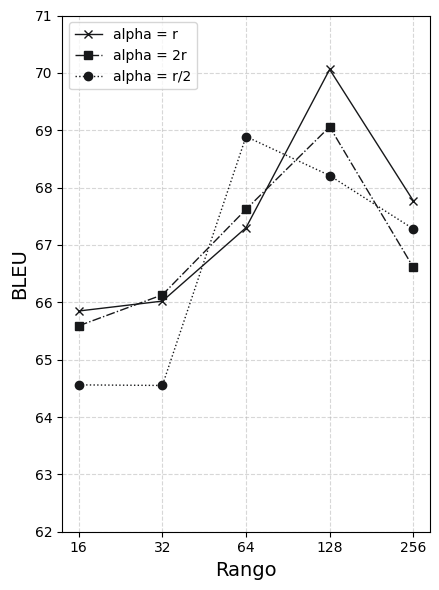
\includegraphics[width=0.9\linewidth, height=9cm]{images/llama_BLEU_} 
\caption{Resultados de BLEU para Llama3-8B}
\label{fig:subim1}
\end{subfigure}
\begin{subfigure}{0.5\textwidth}
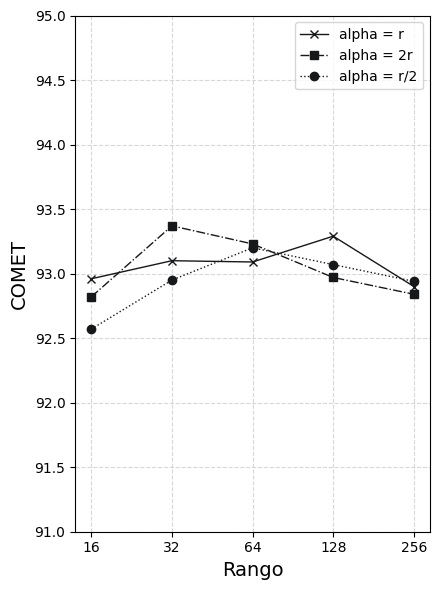
\includegraphics[width=0.9\linewidth, height=9cm]{images/llama_COMET_}
\caption{Resultados de COMET para Llama3-8B}
\label{fig:subim2}
\end{subfigure}

\caption{Resultados de BLEU y COMET obtenidos con el modelo Llama3-8B tras ser entrenado mediante adaptación con LoRA con los valores de $r$ 16, 32, 64, 128 y 256;  y explorando distintas configuraciones de \textit{alpha} con el conjunto de datos en español}
\label{fig:graficasLlama}
\end{figure}

En cuanto a la métrica BLEU, los resultados muestran que todas las configuraciones de \textit{alpha} siguen una tendencia ascendente hasta alcanzar su punto máximo, y a continuación disminuyen la puntuación. En el caso de $\alpha = r/2$, su valor óptimo se alcanza en en $r = 64$. En cambio, con $\alpha = r$ y $\alpha = 2r$ el valor óptimo se encuentra en r = 128. Este comportamiento sugiere que, cuando $\alpha = r/2$, es decir, cuando se da mayor importancia a los parámetros del modelo preentrenado que a los pesos ajustados con LoRA, el aumento del rango tiene un impacto limitado en el rendimiento, ya que no se aprovechan completamente los parámetros libres disponibles con valores de rango superiores a 64. En general, las otras configuraciones de $\alpha$ muestran un desempeño superior, alcanzando su máximo en $r = 128$.

En lo que respecta a la métrica COMET, los resultados muestran que todas las configuraciones de \textit{alpha} tienen valores muy similares, oscilando entre 92.5 y 93.5, y sin mostrar diferencias significativas en su comportamiento.

Así, tanto los resultados de BLEU como de COMET sugieren que la combinación óptima de parámetros es $r = 128$ con $\alpha = r$.

\subsection{Validación del modelo final}

Finalmente, se ha llevado a cabo el entrenamiento del modelo de Llama3 con la mejor combinación de parámetros obtenidos en los experimentos anteriores: $r$ = 128 y $\alpha = r$. En este caso, el modelo ha sido entrenado utilizando todo el conjunto de datos disponible para el experimento de validación cruzada.

Una vez completado el entrenamiento, se ha realizado la evaluación del modelo utilizando el conjunto de datos reservado específicamente para evaluación. De esta manera, se ha evaluado el desempeño del modelo en datos que no habían sido vistos por el modelo en ninguna fase de entrenamiento, lo que proporciona una medida de su capacidad de generalización.

Los resultados obtenidos con esta configuración final han sido los siguientes:

\begin{itemize}
	\item BLEU = 62.90
	\item COMET = 89.15
\end{itemize}

Aunque los valores obtenidos para BLEU y COMET son inferiores a los resultados alcanzados durante la fase de experimentación anterior, estos resultados se encuentran dentro de un rango adecuado de las métricas. En la mayoría de casos, el modelo genera frases que se ajustan bien a las palabras clave proporcionadas, aunque a veces presenta errores relacionados con los tiempos verbales u otras pequeñas confusiones. La disminución en las métricas puede deberse a la diferencia entre el conjunto de entrenamiento y el conjunto de validación. A pesar de esto, los resultados siguen siendo prometedores y reflejan un buen desempeño del modelo en esta tarea.

\subsection{Comparación con los resultados obtenidos mediante \textit{prompting}}

Se ha realizado un experimento adicional para evaluar el modelo Llama3-8B sin entrenamiento previo, con el objetivo de medir la mejora de este tras ser entrenado con el conjunto de datos de entrenamiento. Para ello, se introdujeron al modelo algunos datos específicos mediante
 \textit{prompting}, empleando las técnicas descritas en la Sección \ref{prompting} de \textit{zero-shot prompting} y \textit{few-shot prompting}. La evaluación de estos experimentos se ha realizado utilizando el conjunto reservado para test.

La Tabla \ref{tab:promptingEspañol} resume los resultados obtenidos con las técnicas de \textit{zero-shot prompting} y \textit{few-shot prompting}  y también los resultados del modelo final de Llama3 entrenado mediante LoRA.

\begin{table}[!h]
\caption{BLEU y COMET del modelo Llama3 utilizado mediante \textit{zero-shot prompting}, \textit{few-shot prompting} y entrenamiento mediante LoRA con el conjunto de datos en español}
\begin{center}
\begin{tabular}{ c | c c }
	\ & BLEU & COMET \\
	\hline
	\hline
	\textit{Zero-shot prompting} & 7.17 & 63.69  \\
	\textit{Few-shot prompting} & 47.35 & 87.93 \\
	Modelo final entrenado con LoRA & 62.90 & 89.15 \\

\end{tabular}
\end{center}
\label{tab:promptingEspañol}
\end{table}

En el caso de \textit{zero-shot prompting}, los resultados son realmente bajos y muestran que el modelo no comprende adecuadamente la tarea en la mayoría de los casos. Se identificaron tres tipos de respuesta:

\begin{enumerate}
	\item \textbf{Repetición de las palabras clave}: en la mayoría de casos el modelo se limita a repetir las palabras clave que fueron introducidas, ya sea de manera exactamente igual o con pequeñas modificaciones, como la eliminación de comas, la adición de comillas o el uso de mayúscula en ciertas palabras.
	\item \textbf{Frases sin sentido o sin relación con las palabras clave}: en otros casos, el modelo genera frases utilizando las palabras clave pero que no tienen sentido, o incluso frases que no guardan relación con las palabras introducidas. Por ejemplo, para las palabras clave ``mamá, me, decir, hola, por, mañana´´ el modelo generó la frase ``Mamá, me dice que mañana me voy a comprar un nuevo carro.´´ y para las palabras clave ``no, lo, cambiar´´, generó ``¿Sabes por qué no me gusta el agua?´´.  También hay ocasiones en las que el modelo utiliza las palabras clave para generar las frases pero añade también palabras que no están en la lista de palabras introducidas, generando frases que divagan y no son correctas. Por ejemplo, para las palabras clave ``policía, poner, un, multa´´, la frase esperada era ``El policía puso una multa´´, pero el modelo generó ``La policía pone multas a los conductores que no respetan las normas.´´.
	\item \textbf{Frases similares a las esperadas}: en algunas ocasiones el modelo sí que genera frases que coinciden con las reales o que son similares a estas. Por ejemplo, para los lemas ``qué, llevar, cesta, ?´´ generó correctamente la frase ``¿Qué llevas en la cesta?´´, y para  ``niño, jugar, piscina´´ generó ``El niño juega en la piscina´´, que, aunque no es idéntica a la frase real ``Los niños juegan en la piscina.´´, refleja que el modelo comprendió la tarea.
\end{enumerate}

Para la técnica de \textit{few-shot prompting}, se proporcionaron al modelo cinco ejemplos de palabras clave con sus correspondientes frases generadas. En este caso, el modelo demostró una mejor comprensión de la tarea, generando resultados que, en la mayoría de casos, se acercan más a los reales en comparación con el  \textit{zero-shot prompting}. Sin embargo, presenta mayor cantidad de errores que el modelo entrenado con datos específicos. Algunos de estos errores incluyen cambios en el orden de las palabras, como en el caso de ``mamá, oso, coger, plato, mediano´´, donde el modelo generó ``La mamá coge el plato del oso medio.´´, cuando debería haber generado ``Mamá oso coge el plato mediano.´´. También se observaron casos en los que el modelo añadió palabras que no estaban en la lista de palabras clave. Por ejemplo, para las palabras clave ``este, ser, Caperuza, Roja´´ el modelo generó ``Esta caperucita roja se llamaba María.´´, aunque las palabras ``llamar´´ y ``María´´ no se encontraba en la lista de palabras clave proporcionadas, por lo que no deberían aparecer en la frase.

Los resultados presentados en la Tabla \ref{tab:promptingEspañol} indican que, aunque el \textit{few-shot prompting} produce resultados razonablemente buenos, el entrenamiento realizado al modelo mediante LoRA sí que proporciona una mejora en el rendimiento en comparación con las técnicas de \textit{prompting}. El uso del modelo mediante \textit{zero-shot prompting} presenta grandes limitaciones de comprensión de la tarea. Aunque el \textit{few-shot prompting} mejora los resultados, aún persisten problemas de comprensión en ciertos casos. El modelo entrenado mediante LoRA alcanza resultados mejores en las métricas BLEU y COMET, lo que confirma que el entrenamiento con datos específicos ofrece una mejora frente a los otros.

\section{Experimentos adicionales con el conjunto en inglés}

Para evaluar la influencia del idioma en los resultados de los modelos, se han replicado los mismos experimentos realizados con el conjunto de datos en español utilizando el conjunto en inglés. De nuevo, se han utilizado los modelos Gemma-7B y Llama3-8B disponibles en el portal de \textit{Hugging Face}.

Al igual que en los experimentos anteriores, se ha aplicado la adaptación LoRA y se ha llevado a cabo el entrenamiento utilizando validación cruzada con un total de 10 particiones.

En primer lugar, se han realizado los experimentos para ambos modelos explorando diferentes valores de $r$ (16, 32 y 64) y utilizando una configuración  fija de $\alpha = 2r$. Al igual que con el conjunto en español, los resultados obtenidos con el modelo Gemma son notablemente inferiores a los resultados obtenidos con el modelo Llama3. El mejor valor de rango resultó ser $r = 32$ en ambos casos. En el caso de Gemma, los valores de BLEU y COMET con esta configuración son de 54.32 y 88.88 respectivamente, mientras que los de Llama3 son 62.22 y 91.12.

En la Tabla \ref{tab:comparacionIdiomas} se muestran los mejores resultados obtenidos de BLEU y COMET para cada modelo e idioma. Se han tenido en cuenta los experimentos realizados con los valores de rango 16, 32 y 64 y la configuración de $\alpha = 2r$. En el caso de los experimentos en español, el mejor valor de rango entre estos es $r = 32$ para ambos modelos. Para el conjunto en inglés es $r = 32$ para Llama3 y $r = 16$ para Gemma.

\begin{table}[h]
\centering
\begin{tabular}{c  c | c c}

             &  & BLEU & COMET \\ 
\hline
\hline
& & & \\
 & Llama3 &   66.13   &   93.37    \\
Español &  &      &       \\
 & Gemma  &   52.44   &    88.92   \\
& & & \\
\hline
& & &  \\
 & Llama3 & 62.22    &   91.12    \\
Inglés &  &      &       \\
 & Gemma  &  54.23    &    88.88   \\
& & &  \\
\end{tabular}
\caption{Mejores resultados de BLEU y COMET en los experimentos de ambos idiomas y modelos}
\label{tab:comparacionIdiomas}
\end{table}

\subsection{Exploración de valores de \textit{alpha}}

En los siguientes experimentos, se ha llevado a cabo una exploración de diferentes configuraciones del parámetro \textit{alpha} utilizando el modelo Llama3-8B, ya que este es el modelo que ha demostrado ofrecer mejores resultados.

De manera similar a los experimentos realizados con el conjunto de datos en español, se han probado diferentes valores de rango: 16, 32, 64, 128 y 256. Para cada valor de rango, se han evaluado las siguientes configuraciones de \textit{alpha}: $\alpha = r/2$, $\alpha = r$ y $\alpha = 2r$.

\mycomment{
\begin{table}[!h]
\caption{Puntuación de BLEU y COMET para el modelo Llama3-8B con el conjunto de datos en inglés}
\begin{center}
\begin{tabular}{ c c | c c }
	\hline
	\textit{Rank} & \textit{Alpha} & BLEU & COMET \\
	\hline
	\hline
	16 & 8 & 57.57 & 90.46 \\
	16 & 16 & 59.28 & 90.79 \\
	16 & 32 & 61.84 & 90.86 \\
	\hline
	32 & 16 & 58.97 & 91.10 \\
	32 & 32 & 59.15 & 90.40 \\
	32 & 64 &  62.22 & 91.12 \\
	\hline
	64 & 32 & 60.50 & 90.86\\
	64 & 64 & 61.80 & 90.87\\
	64 & 128 & 63.42 & 90.85\\
	\hline
	128 & 64 & 63.51 & 90.81\\
	128 & 128 & 63.53 & 91.02\\
	128 & 256 & 63.50 & 91.25\\
	\hline
	256 & 128 & 61.69 & 90.57\\
	256 & 256 & 62.98 & 91.01\\
	256 & 512 & 57.20 & 87.68\\	

\end{tabular}
\end{center}
\label{tab: Llama exploración de alpha inglés}
\end{table}
}

Las gráficas de la Figura \ref{fig:graficasLlama inglés} ilustran en el eje horizontal los valores de rango que han sido explorados. En el eje vertical, la gráfica de la izquierda muestra los valores de BLEU, mientras que la de la derecha presenta los valores de COMET. Cada una de las curvas representadas en las gráficas corresponde a una configuración diferente de \textit{alpha}.

\begin{figure}
\begin{subfigure}{0.5\textwidth}
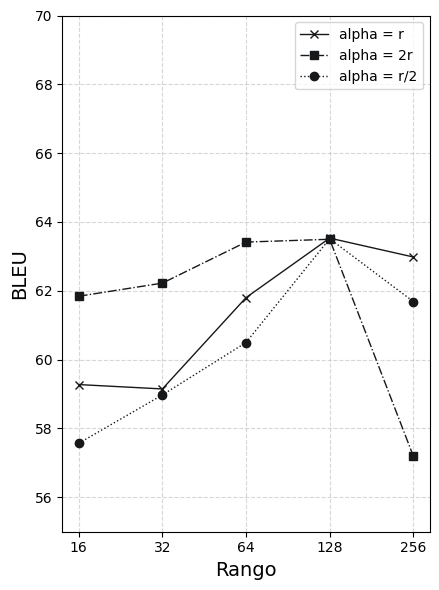
\includegraphics[width=0.9\linewidth, height=9cm]{images/llama_BLEU_en_} 
\caption{Resultados de BLEU para Llama3-8B}
\label{fig:subim1}
\end{subfigure}
\begin{subfigure}{0.5\textwidth}
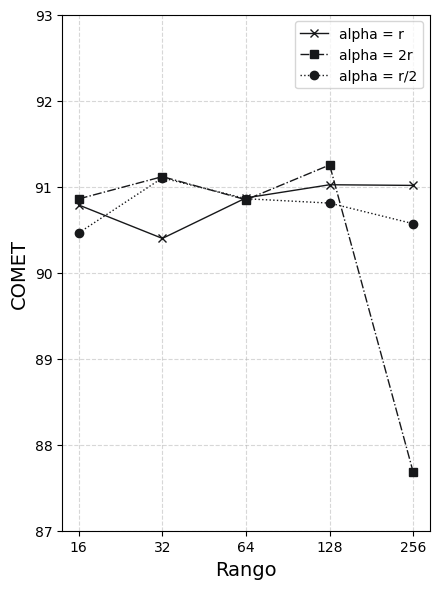
\includegraphics[width=0.9\linewidth, height=9cm]{images/llama_COMET_en_}
\caption{Resultados de COMET para Llama3-8B}
\label{fig:subim2}
\end{subfigure}

\caption{Resultados de BLEU y COMET obtenidos con el modelo Llama3-8B tras ser entrenados mediante adaptación con LoRA con los valores de $r$ = 16, 32, 64, 128 y 256;  y explorando distintas configuraciones de \textit{alpha} con el conjunto de datos en inglés}
\label{fig:graficasLlama inglés}
\end{figure}

Al observar las puntuaciones de BLEU, se puede ver que las tres configuraciones de \textit{alpha} presentan una tendencia ascendente hasta alcanzar su máximo en $r = 128$. Para $r = 256$, los valores de BLEU disminuyen significativamente en los tres casos, de manera similar a lo observado con el conjunto de datos en español. En este caso, la configuración con $r = 128$ y $\alpha = r$ obtiene la mejor puntuación de BLEU, aunque la diferencia con respecto a las otras configuraciones de \textit{alpha} para el mismo valor de $r$ es mínima.

En cuanto a la métrica COMET, las tres configuraciones siguen una tendencia similar a la observada con el conjunto de datos en español. No obstante, se observa un descenso notable en la puntuación de COMET para $r = 256$ y $\alpha = 2r$. El mejor valor de COMET se encuentra en $r = 128$, $\alpha = 2r$.

Considerando ambas métricas, la mejor configuración es $r = 128$, $\alpha = 2r$, ya que ofrece el mejor valor de COMET junto con un buen rendimiento de BLEU.

\subsection{Validación del modelo final}

Igual que con el conjunto en español, el experimento final con los datos en inglés ha consistido en el entrenamiento de un modelo Llama3 utilizando la mejor configuración de parámetros identificada durante la experimentación previa, que fue $r = 128$ y $\alpha = 2r$.

El modelo ha sido entrenado utilizando la totalidad de datos de entrenamiento disponibles. Posteriormente, se ha realizado la validación del modelo utilizando el conjunto de datos de validación que se había reservado desde el inicio de los experimentos. Los resultados obtenidos en las métricas BLEU y COMET han sido los siguientes:

\begin{itemize}
	\item BLEU = 56.70
	\item COMET = 87.96
\end{itemize}

De nuevo, se observa que los resultados obtenidos son inferiores a los obtenidos en los alcanzados en la fase de experimentación anterior. En general, el rendimiento del modelo en inglés es inferior al del modelo en español, cosa que podría deberse a la menor cantidad de datos disponibles en inglés. A pesar de esto, el modelo genera frases muy similares a las reales en la gran mayoría de casos.

\subsection{Comparación con los resultados obtenidos mediante \textit{prompting}}

Al igual que con el modelo en español, se ha llevado a cabo un experimento adicional para evaluar el rendimiento del modelo Llama3-8B en inglés sin entrenamiento previo, con el fin de medir la mejora obtenida tras el entrenamiento. Para ello, se han empleado las técnicas de \textit{zero-shot prompting} y \textit{few-shot prompting}, siguiendo el mismo procedimiento que con los datos en español. Estos experimentos se han evaluado sobre el conjunto en inglés reservado para test.

La Tabla \ref{tab:promptingInglés} muestra los resultados de BLEU y COMET obtenidos con ambas técnicas, así como los resultados del modelo final Llama3 entrenado mediante LoRA con el conjunto de datos de entrenamiento en inglés.

\begin{table}[!h]
\caption{BLEU y COMET del modelo Llama3 utilizado mediante \textit{zero-shot prompting}, \textit{few-shot prompting} y entrenamiento mediante LoRA con el conjunto de datos en inglés}
\begin{center}
\begin{tabular}{ c | c c }
	\ & BLEU & COMET \\
	\hline
	\hline
	\textit{Zero-shot prompting} & 15.36 & 65.80  \\
	\textit{Few-shot prompting} & 55.22 & 88.68 \\
	Modelo final entrenado con LoRA & 56.17 & 87.96 \\

\end{tabular}
\end{center}
\label{tab:promptingInglés}
\end{table}

Al igual que en el caso del modelo en español, los resultados obtenidos con \textit{zero-shot prompting} son significativamente inferiores a los de las otras técnicas, indicando que el modelo tiene grandes problemas para comprender la tarea adecuadamente. En la mayoría de los casos, el modelo se limita a repetir los lemas introducidos, a veces con ligeras variaciones. En muy pocas ocasiones la frase generada por el modelo se asemeja a la frase real.

En el caso del \textit{few-shot prompting}, se proporcionaron al modelo cinco ejemplos de listas de palabras clave con sus correspondientes frases. El modelo muestra un rendimiento mucho mejor, demostrando que es capaz de comprender el objetivo de la tarea. Sin embargo, en algunas ocasiones el modelo añade palabras que no aparecían en la lista de palabras clave. Por ejemplo, para las palabras clave ``snail, become, sad´´, el modelo generó ``The snail becomes sad because of the rain.´´, aunque la palabra ``rain´´ no estaba en el listado. De todas maneras, el modelo generó frases cercanas a las frases reales en la mayoría de ocasiones. Los errores cometidos son similares a los del modelo entrenado con LoRA, y la puntuación de COMET obtenida con \textit{few-shot prompting} es ligeramente superior a la del modelo entrenado con datos específicos.

Así, los resultados de la Tabla \ref{tab:promptingInglés} indican que, aunque el desempeño de \textit{zero-shot prompting} es muy bajo, la \textit{few-shot prompting} resulta muy eficaz. Los resultados obtenidos con esta técnica son muy similares a los obtenidos con el modelo entrenado mediante LoRA en términos de BLEU, y superiores en cuanto a COMET. Esto podría sugerir una posible limitación en la calidad del conjunto de datos en inglés utilizado para el entrenamiento.

\chapter{Análisis posteriores del modelo en español} \label{cap5}

En este capítulo se presentan una serie de análisis y experimentos adicionales que se han llevado a cabo con el objetivo de evaluar de manera más profunda la eficacia del modelo final en español. Este es el modelo Llama3 con $r = 128$ y $\alpha = r$.

En primer lugar, se ha realizado una comparación del rendimiento del modelo con el modelo GPT-4 y la aplicación de AsTeRISCS Grid, ampliamente utilizada en el ámbito de los SAAC. Además, se han realizado experimentos con participantes humanos para verificar si los resultados generados por el modelo son comparables a los obtenidos por personas. Finalmente, se ha realizado un análisis de los errores más comunes cometidos por el modelo, con el fin de identificar áreas de mejora y comprender mejor sus limitaciones.

\section{Comparación con otros modelos} 

Una vez obtenidos los resultados finales del modelo Llama3-8B, se han realizado pruebas adicionales con el modelo GPT-4 y con la aplicación AsTeRICS Grid para comparar su rendimiento. Todas estas pruebas se han realizado utilizando el conjunto de test reservado desde el inicio de los experimentos.

El modelo GPT-4 fue seleccionado para esta comparación debido a su reconocimiento como uno de los modelos de lenguaje grandes más avanzados y potentes disponibles actualmente. Para evaluar su desempeño, se introdujeron los datos de entrenamiento a través de su interfaz \textit{ChatGPT} mediante la técnica de \textit{prompting}, y se le solicitó que generara las frases que se encontraban en el conjunto de test. Es importante destacar que este modelo es significativamente más grande en comparación con Llama3, ya que cuenta con 1.8 trillones de parámetros. Además, no podemos determinar con certeza si GPT-4 ha tenido acceso previo a los datos de test, ya que estos se encuentran accesibles libremente en internet. GPT-4 ha sido entrenado con una gran cantidad de información recopilada de internet, aunque los detalles específicos sobre qué datos han sido utilizados para su entrenamiento no han sido publicados.

Por otro lado, la aplicación AsTeRISCS Grid ha sido incluida en esta evaluación debido a su relevancia como herramienta de comunicación utilizada en el ámbito de los sistemas de comunicación aumentativa y alternativa. Esta aplicación es un comunicador electrónico desarrollado por ARASAAC, que incorpora la función de generar frases conjugadas a partir de las palabras clave introducidas por el usuario. Esta conjugación de las frases se realiza mediante una serie de reglas predefinidas.

La Tabla \ref{tab:comparacionFinal} presenta los resultados de BLEU y COMET obtenidos con los tres modelos (Llama3-8B, GPT-4 y AsTeRISCS Grid).

\begin{table}[!h]
\caption{Puntuaciones de BLEU y COMET de los distintos modelos utilizados para la comparación}
\begin{center}
\begin{tabular}{ c | c c }
	\ & BLEU & COMET \\
	\hline
	\hline
	Llama3 & 62.90 & 89.15  \\
	GPT-4 & 66.36 & 92.51\\
	AsTeRICS Grid & 26.89 & 78.36 \\

\end{tabular}
\end{center}
\label{tab:comparacionFinal}
\end{table}

Observamos que, aunque el modelo entrenado Llama3-8B no alcanza el nivel de rendimiento de GPT-4, sus resultados son notablemente superiores a los de AsTeRICS Grid, una herramienta ampliamente utilizada en el ámbito de los SAAC. Estos resultados sugieren que la integración de modelos de lenguaje grandes podría mejorar significativamente la calidad de las aplicaciones en este campo, proporcionando una alternativa más robusta y efectiva para la generación de frases a partir de las palabras introducidas por los usuarios y mejorando así la calidad de la comunicación de estos.

\section{Experimentos con personas}

Además de las pruebas realizadas con otros modelos, se han realizado también experimentos con un grupo de personas para poder comparar los resultados obtenidos por el modelo Llama3-8B con producciones humanas. Para ello, se explicó la tarea a un grupo de 5 personas, estudiantes de Ciencia de Datos o Informática con edades comprendidas entre 22 y 26 años. A continuación, se les proporcionó el conjunto de datos de entrenamiento para que pudiesen revisar ejemplos de la realización de la tarea, así como el conjunto de datos de validación sin incluir las frases generadas, solamente con las listas de palabras clave.

A partir de esta información, se les pidió a los participantes que escribieran las frases que consideraban que podrían generarse basándose en los ejemplos proporcionados. Posteriormente, se calcularon las puntuaciones de BLEU y COMET para las frases producidas por cada participante, siguiendo el mismo procedimiento utilizado en los experimentos anteriores.

La Figura \ref{fig:comparacionIndividuos} presenta en el eje horizontal los valores de BLEU y en el vertical, los valores de COMET. Los puntos marcados por triángulos representan los resultados obtenidos por los distintos individuos, y el punto marcado con un círculo representa los resultados del modelo.

\mycomment{
\begin{table}[!h]
\caption{Puntuaciones de BLEU y COMET de las personas a las que se le envió la tarea}
\begin{center}
\begin{tabular}{ c | c c }
	\ & BLEU & COMET \\
	\hline
	\hline
	Individuo 1 & 67.95 & 90.26  \\
	Individuo 2 & 70.13 & 92.07\\
	Individuo 3 & 70.63 & 92.08 \\
	Individuo 4 & 62.77 & 90.22 \\
	Individuo 5 & 62.66 & 88.81 \\

\end{tabular}
\end{center}
\label{tab:experimentosPersonas}
\end{table}
}

\begin{figure}[h]
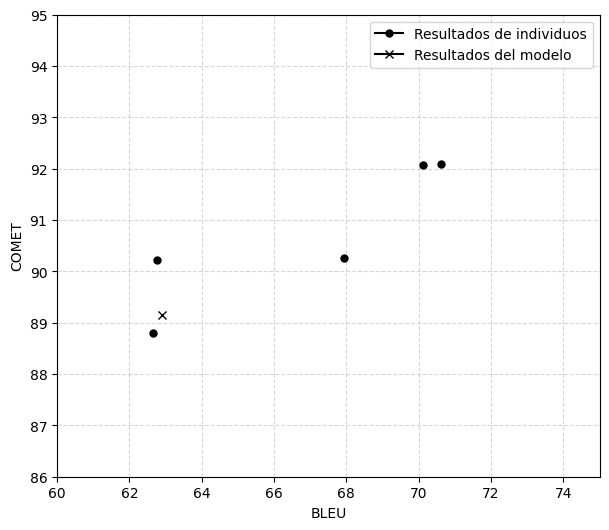
\includegraphics[scale = 0.8]{images/comparacion_individuos.png}
\centering
\caption{Resultados de BLEU y COMET obtenidos por los individuos y por el modelo en la tarea de generación de frases}
\label{fig:comparacionIndividuos}
\end{figure}

Los resultados obtenidos por el modelo final de Llama3 entrenado con el conjunto de datos en español son BLEU = 62.90 y COMET = 89.15. Comparando estos resultados con los obtenidos por personas, observamos que, aunque el modelo Llama3 presenta un rendimiento inferior al promedio de los resultados obtenidos por individuos, supera a dos de ellos en términos de BLEU y a uno en términos de COMET.

Esto sugiere que, a pesar de no alcanzar los niveles más altos de rendimiento humano, el modelo logra generar frases que se acercan a los estándares de calidad que se obtendrían si las frases fueran generadas por personas. Este desempeño cercano a los resultados humanos indica que el modelo Llama3 tiene una capacidad considerable para generar frases de manera efectiva y coherente.

\section{Análisis de errores}

En esta sección se realiza un análisis de los errores más comunes observados en la generación de frases por parte del modelo. El objetivo de este es identificar y comprender los errores recurrentes en las frases generadas, lo que proporcionará una base para futuras mejoras en el proceso.

El análisis se ha realizado comparando las frases generadas del conjunto de validación con las frases reales. Se observa que, de las 50 frases del conjunto, 18 fueron generadas correctamente, es decir, de manera idéntica a las frases reales. Esto significa que el modelo generó un total de 27 frases con algún tipo de error. A continuación se enumeran los errores principales que estas presentan:

\begin{itemize}
	\item \textbf{Errores en los tiempos verbales}: se han identificado 9 frases en las que el único error se relaciona con la conjugación del tiempo verbal. En la Tabla \ref{tab:erroresTiempoVerbal} se presentan tres ejemplos de frases con este tipo de error. Se observa que son casos en los que, a partir de las palabras clave introducidas, resulta muy difícil determinar el tiempo verbal correcto de la frase. El modelo tiende a conjugar las frases en presente, ya que es el tiempo verbal más común, aunque en algunas ocasiones las frases deberían estar en pasado o en futuro. Este error también es frecuente en las generaciones de frases realizadas por personas. La ausencia de pistas claras sobre el tiempo verbal en las palabras clave puede llevar a asumir que el tiempo verbal de la frase debe ser presente.

\begin{table}[!h]
\caption{Frases generadas por Llama3 con errores en el tiempo verbal}
\begin{center}
\begin{tabular}{ c | c | c }
	\ Lemmas & Frase generada & Frase real \\
	\hline
	\hline
	 & & \\
	 no, lo, cambiar & No lo cambio & No lo cambiaré  \\
	 & & \\
	niños, se, reír & Los niños se ríen & Los niños se reían\\
	 & & \\
	perra, tener, cachorros & La perra tiene cachorros & La perra tuvo cachorros \\
	 & & \\

\end{tabular}
\end{center}
\label{tab:erroresTiempoVerbal}
\end{table}

	\item \textbf{Falta de preposición}: en 8 frases, los errores se deben a la falta o confusión de alguna preposición. Se detallan ejemplos de este caso en la Tabla \ref{tab:erroresPreposicion}.

\begin{table}[!h]
\caption{Frases generadas por Llama3 con errores en preposiciones}
\begin{center}
\begin{tabular}{ c | c | c }
	\ Lemmas & Frase generada & Frase real \\
	\hline
	\hline
	 & & \\
	yo, dormir, noche & Yo duermo la noche & Yo duermo por la noche \\
	 & & \\
	Blancanieves, correr, bosque & Blancanieves corre por  & Blancanieves corre \\
	 & el bosque & al bosque \\
	 & & \\
	Juan, se, encontrar, un, mago & Juan se encontró un  & Juan se encontró con \\
	 & mago & un mago \\
	 & & \\

\end{tabular}
\end{center}
\label{tab:erroresPreposicion}
\end{table}

	\item \textbf{Confusión en el sujeto}: un total de 4 frases presentan errores solamente en el sujeto. Los ejemplos de este caso se presentan en la Tabla \ref{tab:erroresSujeto}. Estos errores incluyen la falta del artículo del sujeto debido a que se interpreta el sustantivo como nombre propio.

\begin{table}[!h]
\caption{Frases generadas por Llama3 con errores en el sujeto}
\begin{center}
\begin{tabular}{ c | c | c }
	\ Lemmas & Frase generada & Frase real \\
	\hline
	\hline
	 & & \\
	Ratita, comprar, un, lazo & Ratita compra un lazo & La ratita compra un lazo \\
	 & & \\
	papá, abrir, puerta, de,  & Papá abre la puerta del & El papá abre la puerta del \\
	 coche, con, llave & coche con la llave & coche con la llave \\
	 & & \\
	Ratita, barrer, su, casita & Ratita barre su casita & La ratita barre su casita \\
	 & & \\

\end{tabular}
\end{center}
\label{tab:erroresSujeto}
\end{table}

	\item \textbf{Error en el número}: solo se ha identificado un caso en el que el error radica en el número gramatical. En este caso las palabras clave son `` niño, jugar, piscina ´´. A partir de estas, el modelo generó `` El niño juega en la piscina ´´ en lugar de  `` Los niños juegan en la piscina ´´, que era la frase real. Dado que las palabras clave no especificaban el número, es comprensible que el modelo asumiera el singular. Este error también fue cometido por todos los participantes humanos en el experimento.
\end{itemize}

Las 10 frases restantes presentan varios de los errores mencionados u otros problemas sintácticos. En la Tabla \ref{tab:erroresVariados} se presentan tres ejemplos de frases con distintos errores.

\begin{table}[!h]
\caption{Frases generadas por Llama3 con varios errores}
\begin{center}
\begin{tabular}{ c | c | c }
	\ Lemmas & Frase generada & Frase real \\
	\hline
	\hline
	 & & \\
	 este, ser, Caperuza, Roja & Este ser Caperuza Roja & Esta es Caperuza Roja  \\
	 & & \\
	Reyes, mago, ir, camello & 3 Reyes magos irían & Los Reyes Magos \\
	 & al camello & van en camello \\
	 & & \\
	Caperucita, abuela, ser, feliz & Caperucita es feliz con & Caperucita y la abuela  \\
	 & su abuela & fueron felices \\
	 & & \\

\end{tabular}
\end{center}
\label{tab:erroresVariados}
\end{table}

%\section{Análisis de errores en inglés}



%%%%%%%%%%%%%%%%%%%%%%%%%%%%%%%%%%%%%%%%%%%%%%%%%%%%%%%%%%%%%%%%%%%%%%%%%%%%%%%
%                                 CONCLUSIONS                                 %
%%%%%%%%%%%%%%%%%%%%%%%%%%%%%%%%%%%%%%%%%%%%%%%%%%%%%%%%%%%%%%%%%%%%%%%%%%%%%%%

\chapter{Conclusiones} \label{cap6}

En este trabajo se ha explorado la posibilidad de adaptar modelos de lenguaje grandes a tareas dentro del ámbito de los sistemas de comunicación aumentativos y alternativos. Se han entrenado dos modelos, Gemma y Llama3, utilizando un conjunto de datos en español y en inglés, con el objetivo de generar frases gramaticalmente correctas a partir de una serie de listas de palabras clave o lemas. Estas listas de palabras clave simulan las entradas que los usuarios introducirían a través de la interfaz de un comunicador electrónico.

El modelo Llama3 ha demostrado un rendimiento positivo en este contexto, logrando generar frases bien estructuradas y mostrando resultados muy prometedores y competitivos. Este modelo ha superado a Gemma en términos de precisión y coherencia gramatical. Por su parte, el modelo Gemma ha presentado un rendimiento inferior, lo que sugiere que este modelo tiene una capacidad de adaptación menos efectiva que Llama3.

Aunque los resultados obtenidos con Llama3 han sido satisfactorios, se ha observado que el tamaño del conjunto de datos ha impactado el rendimiento de ambos modelos. A pesar de esta limitación, Llama3 ha demostrado una notable capacidad para adaptarse y generar resultados de calidad.

Estos resultados muestran que los modelos de lenguaje grandes tienen un gran potencial en el campo de la comunicación aumentativa y alternativa. La capacidad de adaptación y el rendimiento prometedor de Llama3 indican que, con conjuntos de datos más extensos y representativos, estos modelos podrían ofrecer soluciones aún más efectivas para mejorar la comunicación de los usuarios con necesidades específicas.

\section{Objetivos cumplidos}

A lo largo del desarrollo de este trabajo, se han cumplido satisfactoriamente los objetivos propuestos inicialmente:

\begin{enumerate}
	\item Se ha realizado una investigación sobre diferentes tipos de SAAC y cómo aplicar herramientas de Aprendizaje Automático e Inteligencia Artificial para mejorar su uso.
	\item Se han adaptado dos modelos de lenguaje grandes de actualidad, Gemma y Llama3, para la tarea de generación de frases sintácticamente correctas a partir de palabras clave para su uso en comunicadores electrónicos. Tras la realización de los experimentos, se determinó que el modelo Llama3 ofrece mejores resultados que Gemma. Los resultados obtenidos resultan prometedores.
	\item Se ha realizado una comparación de los resultados obtenidos con el modelo Llama3 frente al modelo GPT-4 y el comunicador AsTeRISCS Grid. Aunque el modelo desarrollado en este trabajo no supera el rendimiento de GPT-4, demuestra un rendimiento significativamente superior al de AsTeRISCS Grid, lo que muestra que puede suponer un avance importante en este sector.
\end{enumerate}

\section{Propuesta de trabajo futuro}

Aunque los resultados en este trabajo son satisfactorios, se han identificado algunas áreas de mejora que no han podido ser abordadas debido a limitaciones de tiempo, recursos computacionales y costos económicos. Así, para continuar la investigación y mejorar los resultados, se proponen las siguientes líneas de trabajo futuro:

\begin{itemize}
	\item \textbf{Realización de más repeticiones de experimentos}: resultaría interesante realizar más repeticiones de los experimentos realizados para poder obtener resultados más robustos, ya que las variaciones en el entrenamiento pueden influir significativamente en el rendimiento de los modelos. En este proyecto, las limitaciones de tiempo, recursos computacionales y costos económicos han impedido realizar un número más alto de experimentos.
	\item \textbf{Obtención de conjuntos de datos más grandes}: la aplicación de los conjuntos de datos utilizados podría tener un gran impacto positivo en el rendimiento de los modelos de lenguaje. Los conjuntos de datos de los que se disponían eran relativamente pequeños. Un conjunto más grande y diverso permitiría entrenar a los modelos de manera más completa, mejorando su capacidad de generalización y su habilidad para generar frases precisas y apropiadas al contexto.
\end{itemize}

\section{Legado}

Este trabajo supone una contribución al campo de los Sistemas de Comunicación Aumentativa y Alternativa (SAAC). Se ha demostrado que la adaptación de modelos de lenguaje grandes para la generación de frases a partir de palabras clave permite mejorar significativamente la eficacia de estas herramientas, facilitando una comunicación más natural y coherente para las personas que tienen dificultades en esta área.

El código y los datos utilizados están disponibles en el repositorio de GitHub, permitiendo así a otros investigadores reproducir el análisis y trabajo realizado. Toda la documentación relevante está referenciada en la bibliografía.

\section{Relación del trabajo desarrollado con los estudios cursados}

El trabajo desarrollado en este proyecto está estrechamente relacionado con los estudios cursados e integra diferentes competencias y conocimientos adquiridos a lo largo de este. 

En primer lugar, la obtención y transformación de diferentes conjuntos de datos, que es una tarea fundamental de la Ciencia de Datos, han sido necesarios para conseguir los datos para el entrenamiento de los modelos.

El entrenamiento de  modelos de lenguaje grandes, que forma parte del campo del Procesamiento de Lenguaje Natural, se ha basado en conceptos estudiados en la carrera, por ejemplo el \textit{fine-tuning} y la técnica de \textit{cross-validation}.

Se ha profundizado también en técnicas avanzadas como la adaptación de modelos mediante LoRA, una técnica no vista en profundidad durante la carrera pero que ha sido fundamental para el entrenamiento de los modelos en este proyecto.

Por último, el cálculo de métricas y creación de tablas y gráficas han sido cruciales para la interpretación de resultados. Los conceptos de visualización de datos  aprendidos durante los estudios han resultado muy útiles para presentar de manera clara los resultados obtenidos.

En resumen, este proyecto ha permitido aplicar de manera práctica los conocimientos adquiridos en el grado de Ciencia de Datos, desde la preparación de los datos y el entrenamiento de modelos hasta la evaluación y visualización de resultados.


%%%%%%%%%%%%%%%%%%%%%%%%%%%%%%%%%%%%%%%%%%%%%%%%%%%%%%%%%%%%%%%%%%%%%%%%%%%%%%%
%                                BIBLIOGRAFIA                                 %
%%%%%%%%%%%%%%%%%%%%%%%%%%%%%%%%%%%%%%%%%%%%%%%%%%%%%%%%%%%%%%%%%%%%%%%%%%%%%%%

%%%%%%%%%%%%%%%%%%%%%%%%%%%%%%%%%%%%%%%%%%%%%%%%%%%%%%%%%%%%%%%%%%%%%%%%%%%%%%%
%                                BIBLIOGRAFIA                                 %
%%%%%%%%%%%%%%%%%%%%%%%%%%%%%%%%%%%%%%%%%%%%%%%%%%%%%%%%%%%%%%%%%%%%%%%%%%%%%%%

\bibliographystyle{plain}

\bibliography{plantillatfg}

\cleardoublepage

%%%%%%%%%%%%%%%%%%%%%%%%%%%%%%%%%%%%%%%%%%%%%%%%%%%%%%%%%%%%%%%%%%%%%%%%%%%%%%%
%                           APÈNDIXS  (Si n'hi ha!)                           %
%%%%%%%%%%%%%%%%%%%%%%%%%%%%%%%%%%%%%%%%%%%%%%%%%%%%%%%%%%%%%%%%%%%%%%%%%%%%%%%

\appendix

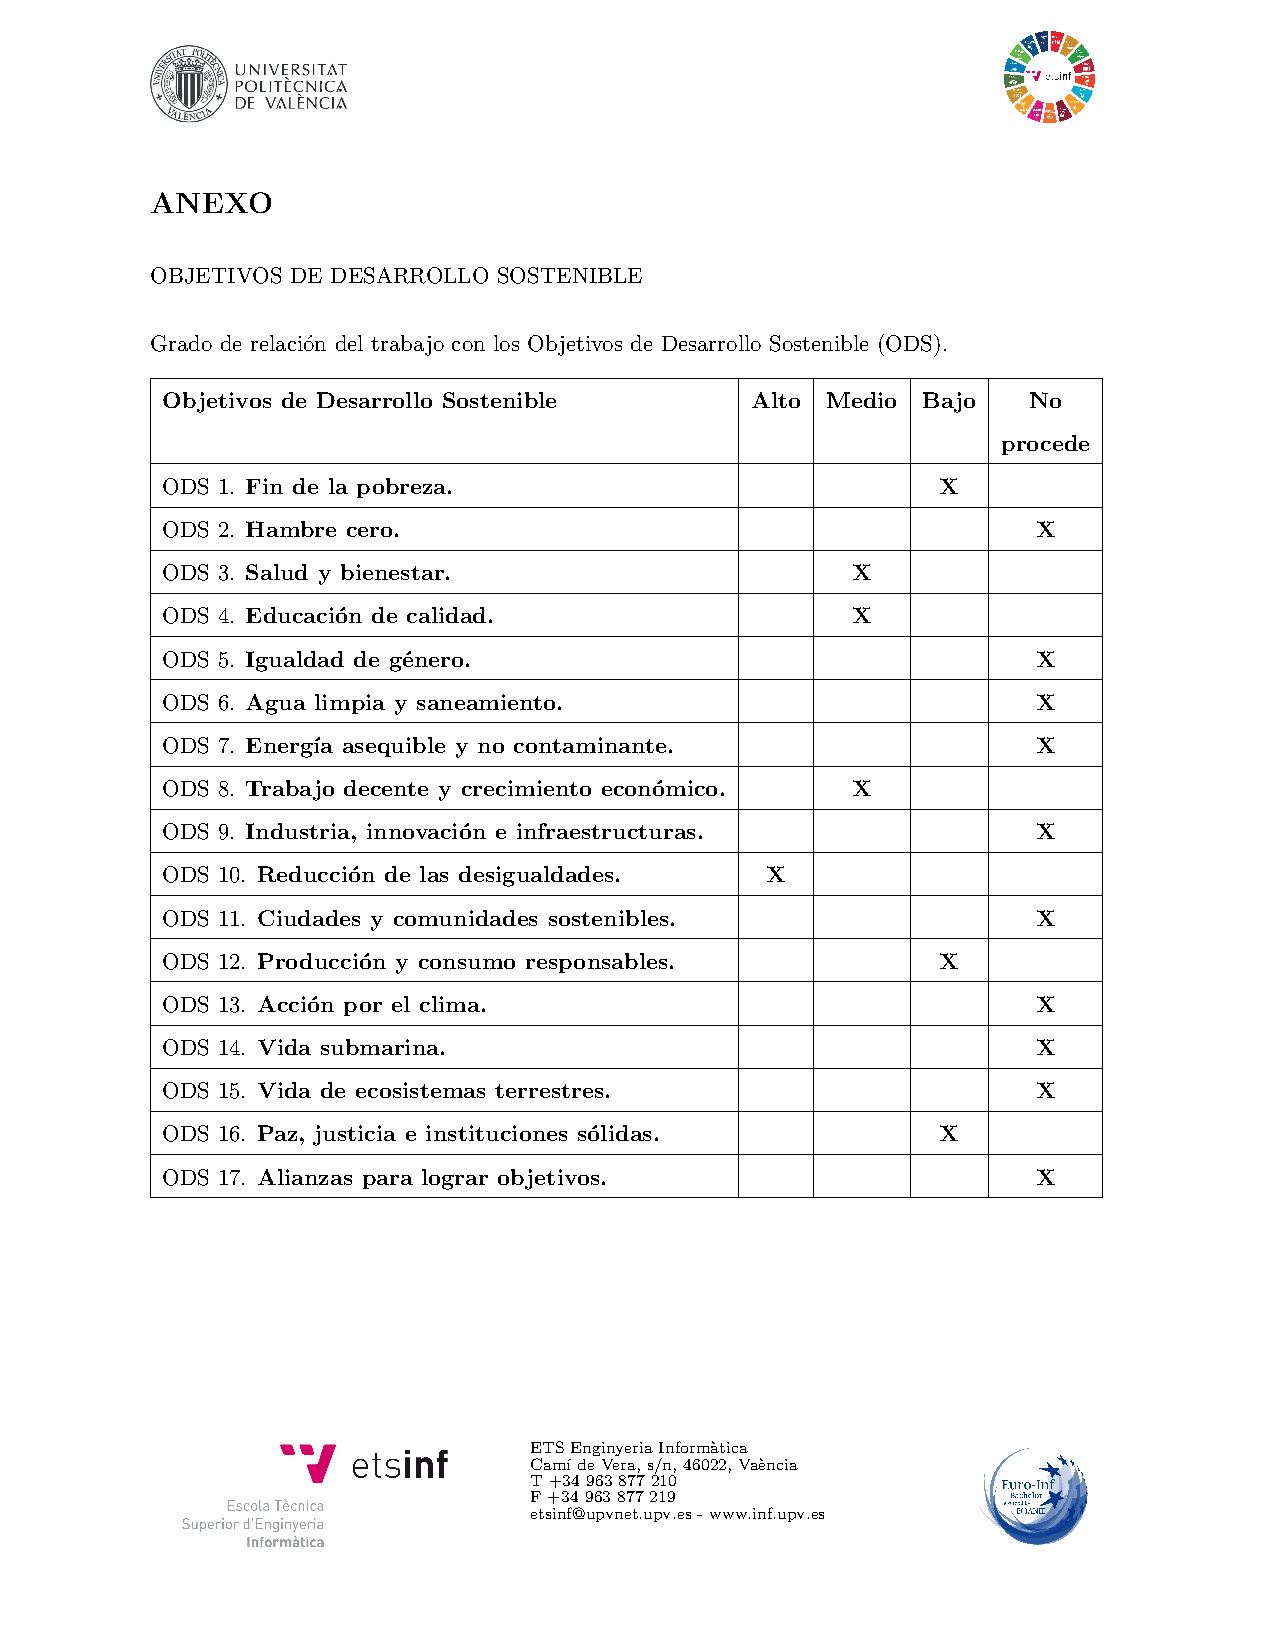
\includepdf[pages=-]{ods_etsinf_anexo.pdf}

%%%%%%%%%%%%%%%%%%%%%%%%%%%%%%%%%%%%%%%%%%%%%%%%%%%%%%%%%%%%%%%%%%%%%%%%%%%%%%%
%                         LA CONFIGURACIO DEL SISTEMA                         %
%%%%%%%%%%%%%%%%%%%%%%%%%%%%%%%%%%%%%%%%%%%%%%%%%%%%%%%%%%%%%%%%%%%%%%%%%%%%%%%

%\chapter{Configuració del sistema}

%\section{Fase d'inicialització}

%\section{Identificació de dispositius}

%%%%%%%%%%%%%%%%%%%%%%%%%%%%%%%%%%%%%%%%%%%%%%%%%%%%%%%%%%%%%%%%%%%%%%%%%%%%%%%
%                               ALTRES  APÈNDIXS                              %
%%%%%%%%%%%%%%%%%%%%%%%%%%%%%%%%%%%%%%%%%%%%%%%%%%%%%%%%%%%%%%%%%%%%%%%%%%%%%%%


%\chapter{??? ???????????? ????}



%%%%%%%%%%%%%%%%%%%%%%%%%%%%%%%%%%%%%%%%%%%%%%%%%%%%%%%%%%%%%%%%%%%%%%%%%%%%%%%
%                              FI DEL DOCUMENT                                %
%%%%%%%%%%%%%%%%%%%%%%%%%%%%%%%%%%%%%%%%%%%%%%%%%%%%%%%%%%%%%%%%%%%%%%%%%%%%%%%

\end{document}
